\documentclass[twosided]{report}
\usepackage{amsmath,amssymb,graphicx}

\setlength{\parindent}{0mm}
\setlength{\parskip}{1em}

\setlength{\textwidth}{171mm}
\setlength{\evensidemargin}{-5mm}
\setlength{\oddsidemargin}{-1mm}

\setlength{\textheight}{229mm}
\setlength{\topmargin}{-16mm}

\def\mathbi#1{\textbf{\em #1}}
\def\BA{\bf{A}}
\def\BB{\bf{B}}
\def\bn{\bf{n}}
\def\CP{\mathcal{P}}
\def\CV{\mathcal{V}}
\def\CI{\mathcal{I}}
\newcommand{\gradt}{\nabla\cdot}

\begin{document}
\begin{center}

{\Large {\bf Twelfth Copper Mountain Conference}} \\
{\large {\bf on}} {\Large {\bf Multigrid Methods}}

{\LARGE {\bf April 3 -- April 9, 2005}}

{\LARGE {\bf Abstracts}}

\end{center}

%%%%%%%%%%%%%%%%%%%%%%%%% INDEX begin


% \begin{itemize}
% \item David Alber,
% {\em Modifying CLJP Coarse Grid Selection to Attain Lower Complexities},
% p.\pageref{alber}
% \item Markus Berndt, J. David Moulton, Glen Hansen,
% {\em Toward an efficient nonlinear solver for an mesh smoothing problem},
% p.\pageref{berndt}
% \item Martin Bedrzins, Christopher Goodyer,
% {\em Efficient parallelisation of a multigrid multilevel integration EHL solver},
% p.\pageref{bedrzins}
% \item Tim Boonen, Stefan Vandewalle,
% {\em A new prolongator for multigrid for the curlcurl equation},
% p.\pageref{boonen}
% \item James Brannick, Marian Brezina, David Keyes, Oren Livne, Irene Livshits, Scott MacLachlan, Tom Manteuffel, Steve McCormick, John Ruge, Ludmil Zikatanov,
% {\em Adaptive Algebraic Multigrid Preconditioners in Quantum Chromodynamics},
% p.\pageref{brannick}
% \item Susanne C. Brenner,
% {\em Multigrid Algorithms for $C^0$ Interior Penalty Methods for Fourth Order Problems},
% p.\pageref{brenner}
% \item Marian Brezina, J.~Brannick, R.~Falgout, S.~MacLachlan, T.~Manteuffel, S.~McCormick, J.~Ruge,
% {\em Application of the Adaptive Smoothed Aggregation to Problems with Nonsmooth Kernels},
% p.\pageref{brezina}
% \item Tim Chartier, Edmond Chow,
% {\em Algebraic Multigrid Schemes},
% p.\pageref{chartier}
% \item Zhen Cheng, Eric de Sturler,
% {\em Effective adaptive multigrid for strongly anisotropic problems with Krylov smoothers},
% p.\pageref{cheng}
% \item Joel E. Dendy, J. David Moulton,
% {\em A Robust Multigrid Method with Cell-Based Coarsening},
% p.\pageref{dendy}
% \item Hans De Sterck, Ulrike Meier Yang,
% {\em Study of Aggressive Coarsening and Multipass Interpolation in Algebraic Multigrid},
% p.\pageref{desterck}
% \item Craig C. Douglas, Yalchin Effendiev,
% {\em Dynamic Data-Driven Application Simulations (DDDAS)},
% p.\pageref{douglas}
% \item Robert D. Falgout,
% {\em Sharpening the Predictive Properties of Compatible Relaxation},
% p.\pageref{falgout}
% \item Krzysztof J. Fidkowski, David L. Darmofal,
% {\em $p$-Multigrid Solution of High-Order Discontinuous Galerkin Discretizations of the Euler and Compressible Navier-Stokes Equations},
% p.\pageref{fidkowski}
% \item Scott R. Fulton, Guohua Zhou,
% {\em Multigrid Solvers on Spherical Geodesic Grids},
% p.\pageref{fulton}
% \item Michael W. Gee, Ray S. Tuminaro,
% {\em Nonlinear Nearly Matrix-Free Algebraic Multigrid for Solid Mechanics},
% p.\pageref{gee}
% \item Jean-Marc Gratien, Pierre Bonneau, Rolland Masson, Phillippe Quandalle,
% {\em Using parallel algebraic multi-grid preconditioner in an industrial reservoir simulation software},
% p.\pageref{gratien}
% \item Serge Gratton, Annick Sartenaer, Philippe L. Toint,
% {\em On Recursive Multiscale Trust-Region Algorithms for Unconstrained Minimization},
% p.\pageref{gratton}
% \item U. Hetmaniuk, R. Lehoucq,
% {\em A new Rayleigh quotient minimization algorithm based on algebraic multigrid},
% p.\pageref{hetmaniuk}
% \item Jonathan J. Hu, Ray Tuminaro, Marzio Sala, Marian Brezina,
% {\em Tools for Analyzing Multigrid Performance},
% p.\pageref{hu}
% \item Samuli Ikonen, Jari Toivanen,
% {\em Multigrid Methods for Pricing American Options under Stochastic Volatility},
% p.\pageref{ikonen}
% \item Jim E. Jones,
% {\em Parallel Multigrid on a Beowulf Cluster},
% p.\pageref{jones}
% \item Dongjin Kim, Dan Stanescu,
% {\em $p$-Multigrid for the Nodal Discontinuous Galerkin Approximation},
% p.\pageref{kimd}
% \item Sang Dong Kim,
% {\em A Preconditioner on High-order Finite Element Methods},
% p.\pageref{kimsd}
% \item Jung-Han Kimn, Blaise Bourdin,
% {\em Implementation of An Overlapping Balancing Domain Decomposition Method for Elliptic PDEs on Unstructured Meshes},
% p.\pageref{kimn}
% \item Tzanio V. Kolev, Panayot S. Vassilevski,
% {\em Experiments with Adaptive Element Agglomeration Algebraic Multigrid for H(div) and H(curl).},
% p.\pageref{kolev}
% \item Ilya Lashuk, Merico Argentati, Evgueni Ovtchinnikov, Andrew Knyazev,
% {\em Preconditioned eigensolvers in Hypre and PETSc},
% p.\pageref{lashuk}
% \item Barry Lee, Izaskun Garrido, Gunnar E. Fladmark, Magne S. Espedal,
% {\em A Multilevel Time Parallelization Algorithm},
% p.\pageref{lee}
% \item Alfonso Limon, Hedley Morris,
% {\em A Multilevel Adaptive Solver for the Density-Gradient Equation},
% p.\pageref{limon}
% \item Irene Livshits,
% {\em Multilevel eigenbasis for Schr\"{o}dinger eigenvalue problems},
% p.\pageref{livshits}
% \item Scott MacLachlan,
% {\em Fully Adaptive AMG},
% p.\pageref{maclachlan}
% \item Roland Masson, V\'{e}ronique Gervais,
% {\em Block Preconditioners with Algebraic Multigrid Block Solve in Stratigraphic Modeling for oil exploration},
% p.\pageref{masson}
% \item Dimitri J. Mavriplis,
% {\em Multigrid solution of the lattice Boltzmann equation},
% p.\pageref{mavriplis}
% \item Miriam Mehl, Nadine Dieminger, Christoph Zenger,
% {\em A cache-oblivious self-adaptive full multigrid method},
% p.\pageref{mehl}
% \item A. J. Meir, Irad Yavneh,
% {\em The Action-Dependent Wave Function Problem: Well Posedness and Efficient Numerical Solutions},
% p.\pageref{meir}
% \item J. David Moulton, Scott P. MacLachlan,
% {\em Multilevel Upscaling: Multigrid's Lost Twin},
% p.\pageref{moulton}
% \item Cristian R. Nastase, Dimitri J. Mavriplis,
% {\em High-Order Spectral $hp$-Multigrid Methods on Unstructured Grids},
% p.\pageref{nastase}
% \item Arie de Niet, Fred Wubs,
% {\em Multilevel Preconditioners in Thermohaline Ocean Circulation},
% p.\pageref{niet}
% \item Akira Nishida,
% {\em AMG Preconditioned Conjugate Gradient Type Methods for Nonsymmetric Eigenproblems},
% p.\pageref{nishida}
% \item Luke Olson, Jeff Heys, Tom Manteuffel, Steve McCormick,
% {\em Algebraic Multigrid (AMG) for Higher-Order Finite Elements},
% p.\pageref{olson}
% \item Cornelis W. Oosterlee, Fransisco J. Gaspar, Francisco J. Lisbona,
% {\em Multigrid for a segregated version of the poroelasticity system},
% p.\pageref{oosterlee}
% \item Serguei Ovtchinnikov, Xiao-Chuan Cai, Florin Dobrian, David Keyes,
% {\em A Fully Coupled Implicit Method for A Magnetohydrodynamics Problem},
% p.\pageref{ovtchinnikov}
% \item Joe Pasciak, Jay Gopalakrishnan,
% {\em The convergence of V-cycle multigrid algorithms for axisymmetric Laplace and Maxwell equations},
% p.\pageref{pasciak}
% \item Jonas Persson, Per L\"{o}tstedt, Lina von Sydow, Johan Tysk,
% {\em Space-Time Adaptive Finite Difference Method for European Multi-Asset Options},
% p.\pageref{persson}
% \item Bobby Philip, Michael Pernice,
% {\em Performance of FAC Preconditioners for Multi-Material Equilibrium Radiation Diffusion on Adaptively Refined Grids},
% p.\pageref{philip}
% \item Oliver R\"{o}hrle, Iain Anderson, Andrew Pullan,
% {\em Modeling Jaw and Teeth Mechanics},
% p.\pageref{rohrle}
% \item Ulrich Ruede, Harald Koestler,
% {\em A robust multigrid solver for the Euler-Lagrange equations with non-smooth coefficients},
% p.\pageref{ruede}
% \item J. G. Schmidt, G.Berti, J.Fingberg,
% {\em On the Use of Algebraic Multigrid inside a Non-Linear Finite Element Method for Maxillo-Facial Surgery Simulations},
% p.\pageref{schmidt}
% \item Bert Seynaeve, Stefan Vandewalle, Bart Nicola\"{i},
% {\em Fourier-mode analysis of a multigrid method for PDEs with random parameters},
% p.\pageref{seynaeve}
% \item Amik St-Cyr, Stephen J. Thomas, Martin J. Gander,
% {\em Optimized Preconditioners for High-Order Finite-Elements},
% p.\pageref{stcyr}
% \item Mohit Tandon, Rajesh Rawat, Philip J Smith, Andrew M Wissink, Brian Gunney,
% {\em AMR for Turbulent Buoyant Plumes},
% p.\pageref{tandon}
% \item Stefan Vandewalle, Martin Gander,
% {\em Analysis of a two-level time-parallel time-integration method for ordinary and partial differential equations},
% p.\pageref{vandewalle}
% \item Li Wang, Dimitri J. Mavriplis,
% {\em Implicit Solution of High-Order Accurate Discontinuous Galerkin Discretizations of the Unsteady Wave Equation Using Spectral Multigrid},
% p.\pageref{wang}
% \item Irad Yavneh, Iddit Shalem,
% {\em Multilevel two-dimensional phase unwrapping},
% p.\pageref{yavneh}
% \end{itemize}


%%%%%%%%%%%%%%%%%%%%%%%%% INDEX end

\begin{center}
\rule{6in}{1pt}
\end{center}

\begin{center}
{\large			\label{alber}
{\bf Modifying CLJP Coarse Grid Selection to Attain Lower
Complexities}

David Alber} \\
Siebel Center for Computer Science \\ University of Illinois at
Urbana-Champaign \\ 201 North Goodwin Avenue \\ Urbana IL 61801
\\
{\tt alber@uiuc.edu}
\end{center}

To build an efficient parallel algebraic multigrid (AMG) solver both
the setup phase and the solve phase need to be implemented with
parallel algorithms.  Parallelizing the latter is straightforward
because of the similarities between the AMG solve phase and geometric
multigrid.  However, parallelizing the original Ruge-St\"{u}ben (RS) setup
phase presents difficulties.  The RS coarse grid selection algorithm
uses a breadth first search for its first pass which makes the
algorithm inherently sequential.  Parallel coarse grid selection
algorithms had to be designed in order to make a parallel setup phase.

Of those algorithms which select coarse grids for use with RS
interpolation, Cleary-Luby-Jones-Plassmann (CLJP) is unique because it
produces the same coarse grid regardless of the number of processors on
which the coarsening algorithm is run.  Additionally, CLJP is able to
coarsen the grid to a single node.  Both of these properties have
positive implications in the design of a parallel setup phase.
Unfortunately, CLJP tends to select coarse grids which lead to high
operator complexities on many problems and especially high complexities
on problems in three dimensions.

This talk discusses methods to modify CLJP in order to produce grid
hierarchies which lead to lower operator complexities.  In particular,
methods to modify the maximal independent set algorithm on which CLJP
is based are examined.  By modifying this algorithm, CLJP can be made
to produce results with more evenly distributed coarse nodes.
Experimental results show that these changes lead to lower operator
complexities.  The eventual goal is to create CLJP-based algorithms
with performance close to that of the Falgout hybrid algorithm while
retaining the positive aspects of the original CLJP.


\begin{center}

\rule{6in}{1pt}
\end{center}

\begin{center}
{\large			\label{berndt}
{\bf
Toward an efficient nonlinear solver for an mesh smoothing problem
}

Markus Berndt} \\
Los Alamos National Laboratory
\\
Los Alamos NM 87545
\\ {\tt
berndt@lanl.gov
}
\\
J. David Moulton, Glen Hansen
\end{center}

The problem of unstructured mesh smoothing can be approached by solving
a set of Laplace-Beltrami equations that are discretized using finite
elements. The resulting discrete problem is non-linear and a
Newton-Krylov type procedure can be employed to solve it. We will
report on our efforts to speed up the solution of this problem using an
AMG based preconditioner in the Krylov step.

\begin{center}

\rule{6in}{1pt}
\end{center}

\begin{center}
{\large			\label{bedrzins}
{\bf
Efficient parallelisation of a multigrid multilevel integration EHL
solver
}

Martin Bedrzins} \\
SCI Institute, Utah
\\
Salt Lake City UT 84112
\\ {\tt
mb@sci.utah.edu
}
\\
Christopher Goodyer
\end{center}

The numerical solution of large scale elastohydrodynamic lubrication
(EHL) problems is only computationally realistic on fine meshes by
making using using multilevel techniques.  In this work we show how the
parallelisation of both multigrid and multilevel multi-integration for
these problems may be accomplished without damaging solution quality.
A parallel performance model of the implemented algorithm is described
and analyzed using the Isoefficiency and Isomemory metrics for
distributed memory architectures.  Results are shown with good
speed-ups and excellent scalability.

Parallelisation of scientific engineering codes, such as the EHL code
considered here, has proved to be particularly useful whenever either
results are needed quickly or the memory requirements are too large to
be handled in serial. In the case of solvers for the important
engineering problem of elastohydrodynamic lubrication both these
situations can arise. The EHL regime occurs in journal bearings and
gears, where, under severe loads in the presence of a lubricant, there
may be a very large pressure exerted on a very small area, often up to
3 GPa.  This causes the shape of the contacting surfaces to deform and
flatten out at the centre of the contact.  There are also significant
changes in the behavior of the lubricant in this area, for example it
may take on glass-like properties.

The computational challenge in solving such problems is considerable.
The equations to be solved consist of a nonlinear differential equation
which is elliptic/hyperbolic and defined in terms of pressure film
thickness values and a coupled integral equation which defines the film
thickness in terms of all the spatial pressures.  The efficient serial
solution of these problems is achieved by using a multigrid solver for
the differential equation coupled to a multilevel multi-integration
method for the film thickness calculation. Although the time dependent
partial differential and integral equations apply only in one or two
space dimensions, they have a dense sparsity pattern and are highly
nonlinear.  Full details of both the EHL problem and the serial
solution methods used are described in the book by Venner and Lubrecht
and with details specific to the discussion here given by the thesis of
Goodyer.

One  of the EHL problems of current interest is to calculate the
frictional characteristics of measured surface roughness profiles.
This has been successfully undertaken for one dimensional line contact
cases.  Tackling the more realistic 2-D case has been recognized as one
of the immediate challenges in tribology. In order to do this spatial
meshes of $10^6 \times 10^6$ points may be needed. This means that
$10^{12}$ dense nonlinear equations need to be solved. This challenge
is beyond a single workstation at present and requires the use of
parallel computers.

In order to describe the parallel solution techniques the numerical
problem to be solved and the serial algorithm will first be described.
The multigrid and multilevel techniques used will be highlighted, along
with the reasons why they make effective parallelisation such a
communication intensive process.  The parallel approaches we have taken
are then explained and a careful performance model constructed using
the isomemory and isoefficiency metrics.  This analysis  will show how
a demanding numerical problem, which is both highly intensive in terms
of communication, and requires global knowledge, has been successfully
parallelised.  Use of MPI has meant this implementation is portable
between both shared and distributed memory architectures.
Communication costs have been limited through use of non-blocking local
directives, and the memory requirements per process have been
significantly reduced.  The computational results show the overall
speed-up of the code is excellent, especially on higher grid
resolutions.  The scalability has been shown to be similarly impressive
with comparable results when increasing the problem size and number of
processors whilst utilising the same coarsest multi-level
multi-integration level.  The paper concludes by considering future
directions in terms of solving still larger problems.



\begin{center}

\rule{6in}{1pt}
\end{center}

\begin{center}
{\large			\label{boonen}
{\bf
A new prolongator for multigrid for the curlcurl equation
}

Tim Boonen} \\
Computer Science Department
\\
Katholieke Universiteit Leuven
\\ {\tt
tim.boonen@cs.kuleuven.ac.be
}
\\
Stefan Vandewalle
\end{center}

We consider algebraic multigrid methods for the numerical solution of
curlcurl systems in computational electromagnetics. Existing
prolongation schemes for the curlcurl equation are often based on the
Reitzinger-Sch\"{o}berl prolongator presented in [1]. There, a
piecewise constant edge prolongator $P_e$ is derived from a piecewise
constant nodal prolongator $P_n$, such that the commutation property is
satisfied. This prolongation scheme can be improved by applying ideas
of smoothed aggregation multigrid to it ([2], [3]).

We will present an alternative prolongation scheme that takes as a
starting point an arbitrary partition of unity nodal prolongator $P_n$.
We will show that it is possible to associate with the set of coarse nodal
elements (the columns of $P_n$) a set of coarse edge elements. The link
between both sets is the analytical formula for edge elements on
triangular/tetrahedral meshes

$$ E_{ij} = N_i \nabla(N_j) - N_j \nabla(N_i)  $$

We will show that in the coarse setting, this formula has an exact
discrete counterpart, which satisfies the commutation property. This
prolongation schema contains the Reitzinger-Sch\"{o}berl edge
prolongator as the special case for a piecewise constant nodal
prolongator $P_n$.


[1] S. Reitzinger, J. Sch\"{o}berl, \emph{An algebraic multigrid method
for finite element discretizations with edge elements}, Numer. Linear
Algebra Appl. 2002, {\bf 9}, pp.223--238.

[2] P.B.Bochev, C.J.Garasi, J.J.Hu, A.C.Robinson, R.S.Tuminaro,
\emph{An
improved algebraic multigrid method for solving Maxwell's equations},
Siam Journal on Scientific Computing, {\bf 25}, pp.623--642, 2003.

[3] J.Hu, R.Tuminaro, P.Bochev, C.J.Garasi, A.Robinson, \emph{Toward an
$h$-independent Algebraic Multigrid Method for Maxwell's Equations},
to appear in SIAM Journal on Scientific Computing, 2005.


\begin{center} \rule{6in}{1pt} \end{center}
\newpage	% H

\begin{center}
{\large			\label{brannick}
{\bf
Adaptive Algebraic Multigrid Preconditioners in Quantum Chromodynamics
}

James Brannick} \\
Dept. of Applied Mathematics
\\
University of Colorado
\\
Boulder CO 80309-0526
\\ {\tt
james.brannick@colorado.edu
}
\\
Marian Brezina, David Keyes, Oren Livne,
Irene Livshits, Scott MacLachlan, Tom Manteuffel,
Steve McCormick, John Ruge, Ludmil Zikatanov
\end{center}


Standard algebraic multigrid methods assume explicit knowledge of
so-called algebraically-smooth or near-kernel components, which loosely
speaking are errors that give relatively small residuals.  Tyically,
these methods automatically generate a sequence of coarse problems
under the assumption that the near-kernel is locally constant.  The
difficulty in applying algebraic multigrid to lattice QCD is that the
near-kernel components can be far from constant, often exhibiting
little or no apparent smoothness. In fact, the local character of these
components appears to be random, depending on the randomness of the
so-called "gauge" group. Hence, no a priori knowledge of the local
character of the near-kernel is readily available.

This talk proposes adaptive algebraic multigrid (AMG) preconditioners
suitable for the linear systems arising in lattice QCD.  These methods
recover good convergence properties in situations where explicit
knowledge of the near-kernel components may not be available.  This is
accomplished using the method itself to determine near-kernel
components automatically, by applying it carefully to the homogeneous
matrix equation, $Ax=0$.  The coarsening process is modified to use and
improve the computed components. Preliminary results with model 2D QCD
problems suggest that this approach yields optimal multigrid-like
performance that is uniform in matrix dimension and gauge-group
randomness.


\begin{center}

\rule{6in}{1pt}
\end{center}

\begin{center}
{\large			\label{brenner}
{\bf
Multigrid Algorithms for $C^0$ Interior Penalty Methods for Fourth Order
Problems
}

Susanne C. Brenner} \\
Department of Mathematics
\\
University of South Carolina
\\
Columbia SC 29208
\\ {\tt
brenner@math.sc.edu
}
\end{center}

Multigrid algorithms for $C^0$ interior penalty methods (which are
discontinuous Galerkin methods) for fourth order problems will be
discussed. We will show that the convergence behavior of the multigrid
algorithms is similar to that for second order problems, provided that
we use a smoothing scheme involving a Poisson solve as a
preconditioner. Such a preconditioner can be easily implemented because
the $C^0$ finite element spaces are standard spaces for second order
problems.


\begin{center} \rule{6in}{1pt} \end{center}
\newpage	% H


\begin{center}
{\large			\label{brezina}
{\bf
Application of the Adaptive Smoothed Aggregation to Problems with
Nonsmooth Kernels
}

Marian Brezina} \\
Dept. of Applied Mathematics
\\
University of Colorado
\\
Boulder CO 80309-0526
\\ {\tt
mbrezina@math.cudenver.edu
}
\\
J.~Brannick,
R.~Falgout,
S.~MacLachlan,
T.~Manteuffel,
S.~McCormick,
J.~Ruge
\end{center}

The success of multigrid methods relies on complementarity between the
relaxation processs and the coarse-grid correction. Multigrid methods
are usually designed based on the assumption that the error that needs
to be eliminated by the coarse-grid correction possesses smoothness.

We discuss several applications of practical interest where these
assumptions are violated, so standard approaches cannot be successfully
applied. We describe the recently developed extension of the smoothed
aggregation method, designed to identify the critical error components
and to incorporate them into the coarse space design. The presented
numerical experiments demonstrate that the method can be used to
achieve good convergence.

\begin{center}


\rule{6in}{1pt}
\end{center}

\begin{center}
{\large			\label{chartier}
{\bf
Algebraic Multigrid Schemes
}

Tim Chartier} \\
Department of Mathematics
\\
Davidson College
\\
Davidson NC 28035-6908
\\ {\tt
tichartier@davidson.edu
}
\\
Edmond Chow
\end{center}

Considerable efforts in recent multigrid research have concentrated on
algebraic multigrid schemes. A vital aspect of this work is uncovering
algebraically smooth error modes in order to construct effective
multigrid components. Many existing algebraic multigrid algorithms rely
on assumptions regarding the nature of algebraic smoothness. For
example, a common assumption is that smooth error is essentially
constant along `strong connections'. Performance can degrade as smooth
error for a problem differs from this assumption. Through tests on the
homogeneous problem
($\mathbi{Ax} = \mathbf{0}$)
adaptive multigrid methods expose
algebraically smooth error.

The method presented in this talk uses relaxation and subcycling on
complementary grids as an evaluative tool in correcting multigrid
cycling. Each complementary grid is constructed with the intent of
dampening a subset of the basis of algebraically smooth error. The
particular implementation of this framework manages smooth error in a
manner analogous to spectral AMGe. Numerical results will be included.


\begin{center} \rule{6in}{1pt} \end{center}
\newpage	% H

\begin{center}
{\large			\label{cheng}
{\bf
Effective adaptive multigrid for strongly anisotropic problems with
Krylov smoothers
}

Zhen Cheng} \\
Department of Computer Science
\\
University of Illinois
\\
Urbana IL 61801
\\ {\tt
zcheng@uiuc.edu
}
\\
Eric de Sturler
\end{center}

We consider the parallel solution of strongly anisotropic diffusion
problems on adaptive grids by multigrid methods. The standard multigrid
methods with pointwise relaxation and standard coarsening have problems
because smoothers are not effective. To improve multigrid, the common
ways are to use semicoarsening or line smoothers. However, neither of
these techniques is suitable for parallel adaptive grids environment.
Moreover, both techniques require that the anisotropy aligned with the
grid, which may not be the case for realistic problems. In this talk,
we will discuss a robust and easy-to-parallelize smoother for multigrid
which can deal with strongly anisotropic problems on adaptive grids
effectively. This method remains effective even if the anisotropy is
not aligned with the grid.

We use multilevel adaptive technique (MLAT). The main idea of MLAT is
to perform smoothing sweeps only on locally refined grids, and use the
full approximation scheme (FAS) to generate the error correction cycle.
We propose to use Krylov subspace methods as smoothers. Our numerical
experiments show that they reduce oscillatory error components
effectively. Therefore with such smoothers, multigrid achieves fast
convergence rate. Moreover, parallelizing Krylov methods is
straightforward since only matrix vector products and vector inner
products need communication.

Convergence rate analysis for multigrid on adaptive grids can be
simplified to analysis on uniform grids, since with properly chosen
interpolation and prolongation operators, convergence rate on adaptive
grids is almost identical to that on uniform grids. Standard analytic
tools such as Local Fourier Analysis (LFA) fail for Krylov smoothers
because they require the smoothing operators to be linear. In addition,
Krylov methods are not ``strict'' smoothers. Their smoothing effect for
high frequency modes may deteriorate when large smooth error components
are present. In our work, we use a slightly different approach. Assume
the coarse grid correction operator (including interpolation and
restriction) satisfies certain requirements, we derive the
level-independent upper bound for convergence rate of Krylov methods.
This rate is used to estimate multigrid convergence rate. This explains
why level-independent convergence rate of multigrid is achieved. The
numerical experiments verify our statement. Our approach of
quantitative analysis can be applied to more general problems and may
be useful for other multigrid practitioners.

This work is part of IBEAM project which is sponsored under a Round III
Grand Challenge Cooperative Agreement with NASA's Computational
Technologies Project.


\begin{center} \rule{6in}{1pt} \end{center}
\newpage	% H


\begin{center}
{\large			\label{dendy}
{\bf
A Robust Multigrid Method with Cell-Based Coarsening
}

Joel E. Dendy} \\
MS B284
\\
Los Alamos National Laboratory
\\
Los Alamos NM 87544
\\ {\tt
jed@lanl.gov
}
\\
J. David Moulton
\end{center}

Generally robust multigrid codes, like BoxMG, employ Galerkin
coarsening to form the coarse grid operators. That is, if the fine
grid operator is $A$, then the coarse grid operator is $RAP$, where
$P$ is the interpolation operator from the coarse grid to the fine
grid, and $R$ is the restriction operator from the fine grid to the
coarse grid. In BoxMG, $R$ is chosen as the transpose of $P$. This choice
minimizes the error in the range of interpolation. Also, in BoxMG,
interpolation is operator-induced, thereby approximately preserving
the continuity of the normal component of the flux across interfaces.
Cell-centered discretizations on a logically structured grids are
readily treated with BoxMG by associating them with the corresponding
dual grid. However, this approach does not preserve the cell based
structure on coarser levels. Although this structure may not be
important in some applications, in the case of patch- or cell-based
mesh refinement, it is very desirable.

Several multigrid methods have
been proposed to coarsen by cells, but these methods have been either
too costly or not robust with respect to fine-scale discontinuous
coefficients. For example coarsening by cells, using an
operator-induced piecewise bilinear interpolation for $P$, the transpose
of $P$ for $R$, and forming the coarse grid operator as $RAP$ leads to
unacceptable stencil growth. In contrast, Wesseling has investigated a
method that coarsens by cells, in which $R$ is not the transpose of $P$,
yet under certain conditions RAP is symmetric; however, his use of a
non-operator-dependent $P$ yields a method that is not as robust as
BoxMG. In this paper we explore the use of multiple dual-meshes on a
logically structured two-dimensional grid in conjunction with the
variational framework of BoxMG to create a robust method that coarsens
by cells while maintaining a 9-point coarse-grid operator on all
levels. This approach readily extends to the cases of patch- and
cell-based refinement.

\begin{center}

\rule{6in}{1pt}
\end{center}

\begin{center}
{\large			\label{desterck}
{\bf
Study of Aggressive Coarsening and Multipass Interpolation in Algebraic
Multigrid
}

Hans De Sterck} \\
Department of Applied Mathematics
\\ University of Waterloo \\
Ontario, Canada
\\ {\tt
hdesterck@uwaterloo.ca
}
\\
Ulrike Meier Yang
\end{center}

Algebraic multigrid is a very efficent algorithm for solving large
linear systems on unstructured grids. Use of coarsening schemes such as
parallel variants of the standard coarsening algorithm by Ruge and
Stueben [1] or CLJP coarsening [2], a method based on parallel maximal
independent set algorithms, can lead to high complexities with regard
to memory usage as well as computation time, which adversely affect
scalability.
In recent work [3], we have proposed two new parallel AMG coarsening
schemes, that are based on solely enforcing a maximum independent set
property, resulting in sparser coarse grids. The new coarsening
techniques remedy memory and execution time complexity growth for
various large three-dimensional (3D) problems. If used within AMG as a
preconditioner for Krylov subspace methods, the resulting iterative
methods tend to converge fast. For some difficult problems, however,
these methods still produce complexities that are too high, or don't
converge well enough, and further remedies in terms of coarsening and
interpolation need to be found in order to obtain scalable methods.
In this paper we describe the combination of these various coarsening
methods with ``aggressive coarsening'' techniques, which require long
range ``multipass'' interpolation [4], and empirically study complexity
and convergence properties of the resulting iterative methods. The
resulting AMG methods, implemented in the hypre solver library [5], are
applied to first-order system least-squares (FOSLS) discretizations of
elliptic PDE systems. Parallel scalability of the combined FOSLS-AMG
method is investigated for large-scale three-dimensional applications.

*This work was performed under the auspices of the U.S. Department of
Energy by University of California Lawrence Livermore National
Laboratory under contract number W-7405-Eng-48 and subcontract number
B545391.

[1] J. Ruge, K. Stueben, Algebraic multigrid (AMG), in: S. McCormick,
ed., Multigrid Methods, vol. 3 of Frontires in Applied Mathematics
(SIAM, 1987) 73--130.

[2] V. E. Henson, U. M. Yang,
{\em BoomerAMG: a Parallel Algebraic Multigrid
Solver and Preconditioner}, Applied Numerical Mathematics,
{\bf 41} (2002) 155--177.

[3] H. De Sterck, U. M. Yang, and J. J. Heys,
{\em Reducing Complexity in
Parallel Algebraic Multigrid Preconditioners}, submitted to SIAM Journal
on Matrix Analysis and Applications, 2004.

[4] K. Stueben, {\em Algebraic multigrid (AMG): an introduction with
applications}, in: U. Trottenberg, C. Osterlee and A. Schueller, eds.,
Multigrid (Academic Press, 2000) 413--532.

[5] R. Falgout, U. M. Yang, {\em hypre: a Library of High Performance
Preconditioners}, in Computational Science - ICCS 2002 Part III, P.
Sloot, C. Tan, J. Dongarra and A. Hoekstra, eds., Lecture Notes in
Computer Science, {\bf 2331} (Springer, 2002) 632--641.

\begin{center}

\rule{6in}{1pt}
\end{center}

\begin{center}
{\large			\label{douglas}
{\bf
Dynamic Data-Driven Application Simulations (DDDAS)
}

Craig C. Douglas} \\
Departments of Computer Science and Mechanical Engineering
\\
University of Kentucky, Lexington KY
\\
and
\\
Department of Computer Science \\ Yale University, New Haven CT
\\ {\tt
douglas-craig@cs.yale.edu
}
\\
Yalchin Effendiev
\end{center}

DDDAS is a new paradigm in which data dynamically controls almost all
aspects of long term simulations. Rather than run many simulations
using static data as initial conditions, a very small number of
simulations are run with additional data injected as it becomes
available. Most candidate problems for the DDDAS paradigm involve
solving a nonlinear time dependent partial differential equation of the
form
$F(x+Dx(t))=0$ by iteratively choosing a new approximate
solution $x$ based on the time dependent perturbation
$Dx(t)$.

In practice, the data streaming in may have errors and therefore may
not be completely accurate or reliable (for example, in reservoir data
sets, a 15\% error in the data is common). As a result, perhaps one does
not need to solve the nonlinear equation precisely at each step. This
can expedite the execution.

At each iterative step, the following three issues may need to be
addressed:
\begin{enumerate}
\item Incomplete solves of a sequence of related models must be
understood.
\item The effects of perturbations, either in the data and/or the
model, need to be resolved and kept within acceptable limits.
\item Nontraditional convergence issues have to be understood and
resolved.
\end{enumerate}

Consequently, there will be a high premium on developing quick
approximate direction choices, such as, lower rank updates and
continuation methods, and understanding their behavior are
important issues. Fault tolerant algorithms have a premium.

The dynamic data is used to determine
\begin{enumerate}
\item Whether or not a warm restart is necessary due to
unacceptable errors building up in parts of the domain.
\item If a rollback in time is required.
\item If the simulation is running with acceptable errors.
\end{enumerate}

Ideally, there does not have to be a human in the
control loop throughout a simulation.

Using the data appropriately lets the physical and
mathematical models, the discretization, and the
scales of interesting parts of the computations
become parameters that can be changed during the
course of the simulation. In addition, error
propagation is of particular interest in nonlinear
time dependent simulations.

DDDAS offers interesting computational and
mathematically unsolved problems, such as, how do you
analyze the properties of a generalized PDE when you
do not know either where or what the local boundary
conditions are at any given moment in the simulation
in advance?

\begin{center}

\rule{6in}{1pt}
\end{center}

\begin{center}
{\large			\label{falgout}
{\bf
Sharpening the Predictive Properties of Compatible Relaxation
}

Robert D. Falgout} \\
Lawrence Livermore National Laboratory
\\
P.O. Box 808, L-561
\\
Livermore CA 94551
\\ {\tt
rfalgout@llnl.gov
}
\end{center}

The notion of compatible relaxation (CR) was introduced by Brandt in
[1] as a modified relaxation scheme that keeps the coarse-level
variables invariant. Brandt stated that the convergence rate of CR is a
general measure for the quality of the set of coarse variables. A
supporting theory for these ideas was presented in [2], from which we
developed a CR-based algebraic coarsening algorithm for use in
algebraic multigrid (AMG) methods. In [3], a new sharp convergence
theory was developed for AMG. The form of this new theory bears a
striking resemblance to its predecessor and suggests the possibility of
improving the CR measure.

In this talk, we will use the relationship between these two theories
to motivate a new approach for CR, one that has the potential of being
a sharper measure of coarse grid quality and a better predictor of AMG
convergence (one specific version of this method was suggested by Livne
[4]). We will discuss the theoretical properties of the new method,
provide some numerical results, and discuss open questions and future
directions.

This work was performed under the auspices of the U.S. Department of
Energy by University of California Lawrence Livermore National
Laboratory under contract No. W-7405-Eng-48.

[1] A. Brandt,
{\em General highly accurate algebraic coarsening}, Electronic
Transactions on Numerical Analysis, {\bf 10} (2000), pp.1--20.

[2] R.~D.~Falgout and P.~S.~Vassilevski, {\em On Generalizing the AMG
Framework}, SIAM J.~Numer.~Anal., {\bf 42} (2004), pp.1669--1693.

[3] R.~D.~Falgout, P. S. Vassilevski, L. T. Zikatanov,
{\em On Two-Grid Convergence Estimates},
Numer. Linear Algebra Appl., to appear.

[4] O.~E.~Livne,
{\em Coarsening by Compatible Relaxation},
Numer.~Linear Algebra Appl., {\bf 11} (2004), pp.205--227.

\begin{center}

\rule{6in}{1pt}
\end{center}

\begin{center}
{\large			\label{fidkowski}
{\bf
$p$-Multigrid Solution of High-Order Discontinuous Galerkin
Discretizations of the Euler and Compressible Navier-Stokes Equations
}

Krzysztof J. Fidkowski} \\
Massachusetts Institute of Technology \\
77 Mass. Ave \\
MIT 37-442 \\
Cambridge MA 02139
\\ {\tt
kfid@mit.edu
}
\\
David L. Darmofal
\end{center}

In this talk, we focus on a $p$-multigrid solution algorithm for
high-order discontinuous Galerkin (DG) finite element discretizations
of the Euler and compressible Navier-Stokes equations. $p$-Multigrid, or
multi-order, solution strategies have been studied by other authors,
including Helenbrook, Mavriplis, and most recently Bassi and Rebay.
Common features of this method for high-order DG include ease of
implementation and order-independent convergence rates. A key aspect of
our $p$-multigrid implementation is the use of an element-line Jacobi
smoother instead of the standard element-Jacobi. The element-line
Jacobi smoother consists of solving implicitly on lines of elements
formed using coupling based on a $p=0$ discretization of the scalar
convection-diffusion equation. This choice of elemental coupling allows
for the removal of stiffness associated with strong convection or
regions of high grid anisotropy frequently required in viscous layers.
A line creation algorithm is presented for general unstructured meshes,
showing how unique lines can be obtained in two and three dimensions
for a given elemental coupling.

Using Fourier analysis for scalar convection-diffusion, we demonstrate
that the higher-order DG discretizations can be stably marched for all
orders with element Jacobi and element-line Jacobi schemes without the
use of multi-stage iterations. $p$-Multigrid is then applied with the
element-line smoother to inviscid and viscous test cases, in two and
three dimensions. Results demonstrate optimal order of accuracy of the
discretization, as well as $p$-independent multigrid convergence rates.
$h$-dependence is observed, although it is not found to be strong for
many practical problems. Finally, for the smooth problems considered,
$p$-refinement outperforms $h$-refinement in terms of the time required to
reach a desired high accuracy level.



\begin{center} \rule{6in}{1pt} \end{center}
\newpage	% H


\begin{center}
{\large			\label{fulton}
{\bf
Multigrid Solvers on Spherical Geodesic Grids
}

Scott R. Fulton} \\
Department of Mathematics
\\
Clarkson University
\\
Potsdam NY 13699-5815
\\ {\tt
fulton@clarkson.edu
}
\\
Guohua Zhou
\end{center}

Spherical geodesic grids offer several attractive features for
geophysical fluid dynamics modeling: quasi-isotropic discretizations
and quasi-uniform resolution (which eliminates the pole problem of
conventional latitude-longitude grids). Modeling fluid flow on such a
grid results in various elliptic problems which must be solved
efficiently, e.g., the Poisson problem relating stream function to
vorticity and modified Helmholtz problems with variable coefficients
arising in semi-implicit time integration.

Heikes and Randall (1995) introduced a multigrid algorithm for the
two-dimensional Poisson problem on a spherical geodesic grid. In this
paper we: (1) provide a smoothing analysis for this method and discuss
possible algorithmic improvements, (2) extend the algorithm to
variable-coefficient problems in two and three dimensions (using an
isentropic vertical coordinate), and (3) provide numerical experiments
showing performance consistent with the analysis. We also illustrate
the use of these multigrid solvers in a three-dimensional dynamical
core for a climate model.

\begin{center}

\rule{6in}{1pt}
\end{center}

\begin{center}
{\large			\label{gee}
{\bf
Nonlinear Nearly Matrix-Free Algebraic Multigrid for Solid Mechanics
}

Michael W. Gee} \\
Sandia National Laboratories
\\
PO Box 5800, MS 1110
\\
Albuquerque  NM  87185-1110
\\ {\tt
mwgee@sandia.gov
}
\\
Ray S. Tuminaro
\end{center}

The increasing demands of large-scale complex solid mechanics
simulations are placing greater emphasis on the challenges associated
with the efficient solution of the set of nonlinear equations. Here,
the solution of large systems of equations with material and geometric
nonlinearities in a parallel framework is addressed.


Instead of applying widely used Newton- or Newton-Krylov type methods
that involve the derivation of a stiffness matrix and a sequence of
linear solves, the presented work details the implementation of a
(nearly) matrix-free nonlinear algebraic multigrid algorithm applied to
solve this set of nonlinear equations.


As a basic iterative method, a nonlinear conjugate gradient algorithm
(nlnCG) using the Polak-Ribiere formula and a secant method for the
step size is applied. It has the advantage of being a completely
matrix-free method eliminating the need to form a stiffness matrix.
Preconditioned nonlinear CG is then applied as a smoother/coarse solver
in a classical full approximation scheme (FAS) nonlinear multigrid
cycle. Transfer operators are constructed by an aggregation approach
operating on the graph of the fine level problem. The preconditioners
to the nlnCG on all levels are obtained by multicolor finite
differencing and are chosen to be either simple Jacobi or a direct
solve on the coarsest level.
For Jacobi-preconditioned nonlinear CG, only the main diagonal of a
Jacobian matrix needs to be formed involving a distance-1 graph
coloring algorithm and an inexpensive modified colored finite
difference scheme.


The algorithm is implemented within Sandia National Laboratories'
freely available parallel `Trilinos' linear algebra framework and makes
use of its smoothed aggregation multigrid library `ML' and its
nonlinear solver library `NOX'. The outline of the algorithm and
implementation are given together with examples demonstrating the
advantages of this new approach. Several variants of the algorithm will
be discussed and compared.

\begin{center}

\rule{6in}{1pt}
\end{center}

\begin{center}
{\large			\label{gratien}
{\bf
Using parallel algebraic multi-grid preconditioner in an industrial
reservoir simulation software
}

Jean-Marc Gratien} \\
Institut Fran\c{c}ais du P\'{e}trole
\\
1 et 4 avenue Bois Pr\'{e}au
\\
92852 Rueil-Malmaison Cedex
\\
France
\\ {\tt
j-marc.gratien@ifp.fr
}
\\
Pierre Bonneau,
Roland Masson,
Phillippe Quandalle
\end{center}

As full field reservoir simulations require a large amounts of
computing resources, the trend is to use parallel computing to overcome
hardware limitations. This paper presents the linear solvers and the
preconditioning techniques applied to solve very large scale problems
in the reservoir simulation software developed at IFP, software which
has been specially designed for Linux clusters. We discuss on the
choice of different efficient preconditioners. We report the
scalability of the parallel simulator and numerical stability of
underlying algorithms calculated from a test campaign on either
synthetical or real industrial study case.

The reservoir simulator is based on a system of partial differential
equations with algebraic closure laws discretized with a finite volume
scheme in space and a fully implicit or semi-implicit time integration.
After a Newton type linearization of the non linear system, we are
left, at each Newton iteration, with the solution of a large, ill
conditioned linear system coupling several unknowns of mixed parabolic
and hyperbolic type. Progress of computer performances now allows to
better take into account physical phenomenon like strong and very
strong rock heterogeneities and anisotropies in reservoir modeling so
that the complexity of reservoir simulations keeps on increasing with
larger meshes, and more difficult problems. This in turn urges the need
to design more efficient and more scalable preconditioned iterative
solvers, adapted to the new parallel architectures, in order to fully
benefit from the computers performances on such complex cases.

Due to the high condition number of the linear system, the convergence
of the Newton algorithm can be very sensitive to the choice of the
preconditioner, to the linear system stopping criteria and even to the
number of processors in parallel implementations. In such cases, the
accuracy of the solver is critical to ensure parallel performance as
the cumulative number of steps (solver resolution, Newton loops, time
loops) can be very dependent on the number of domains and as the cost
of a run depends on this cumulative number of steps. This shows the
importance of choosing a stable numerical scheme, good solver options
and robust parallel preconditioner to have a numerically stable
simulation. This difficulty emphasizes the special importance of using
very stable numerical schemes during parallel simulation. Solver
options may have important influence on convergence criteria, and the
choice of a good parallel preconditioner can help to have stable
convergence iteration numbers.

In the standard sequential simulator, linear systems are efficiently
solved by the Bi Conjugated Gradient Stabilised with an incomplete ILU0
preconditioner. This preconditioner, well known to be efficient for
standard case is not naturally parallel as its algorithm is recursive.

We have developed a new parallel ILU0 preconditioner which turns to be
a good scalable preconditioner. However, it can encounter difficulties
on complex industrial cases with very complex geometry and physical
models. ILU0 is not scalable with respect to the size of the mesh and
the jumps of the permeability field. Multigrid methods are known to be
scalable for scalar convection diffusion problems but it is also known
that they are not adapted to systems coupling unknowns of mixed types.
Our approach is to define a pressure block that will concentrate most
of the bad conditioning and ellipticity of the system, and for which we
shall used a multigrid preconditioner. The definition of this block is
obtained by linear combination of the rows and columns in order to
reduce the coupling with the other variables (compositions and
concentrations). For the remaining variables and equations we use a
block Gauss Seidel approach. In some cases, this approach does not
ensure a sufficient coupling of the variables, and it needs to be
combined mutiplicatively with a global ILU0 preconditioner.

In reservoir modeling, the linear systems couple a pressure unknown of
elliptic or parabolic type to concentrations or saturations unknowns of
hyperbolic type. In some industrial cases, especially when there are a
lot of heterogeneities and anisotropies, we have noticed that the
variations of saturation are very sensitive to pressure gradient so
that having a robust preconditioner for the pressure is very
important. As a consequence, Algebraic Multigrid Methods have to be
considered as good candidates for preconditioning. Thus, we have
developed 2 AMG based preconditioners . The first approach is a Block
Aggregation AMG. It aims at taking advantage of the natural block
structure of the system when the unknowns pressure and saturation are
grouped cell by cell. This strategy turns out to be effective when a
block ILU0 smoother is used in the multigrid cycle. The second approach
called ``Two level AMG'' combines an algebraic multigrid method on
pressure unknowns with a more traditional parallel method on other
variables (ILU0, Block ILU0, polynomial). This results in a new method
which is robust, parallel and efficient

We have tested these methods (Parallel ILU0, Two level AMG and Block
Aggregation AMG) and studied their influence on the performance and on
the numerical stability of the reservoir simulator for different study
case. We discussed the results obtained on a synthetical study case,
the Tenth SPE Comparative Solution Project, Model 2 and on some real
industrial customer study cases.

\begin{center}


\rule{6in}{1pt}
\end{center}

\begin{center}
{\large			\label{gratton}
{\bf
On Recursive Multiscale Trust-Region Algorithms for Unconstrained
Minimization
}

Serge Gratton} \\
CERFACS \\ Toulouse \\ France
\\ {\tt
gratton@cerfacs.fr
}
\\
Annick Sartenaer,  Philippe L. Toint
\end{center}

A large class of large-scale finite-dimensional minimization programs
arises from the discretization of infinite-dimensional problems, such
as optimal-control problems defined in terms of either ordinary or
partial differential equations. We report here on a potentially
efficient new class of algorithms using this structure and briefly
discuss a first set of numerical experiments. A simple first approach
that we refer to as mesh refinement, is to use coarser grids in order
to compute approximate solutions which can then be used as starting
points for the optimization problem on a finer grid (see [2], [3] or
[8], for instance). However, potentially more efficient techniques are
inspired from the multigrid paradigm in the solution of partial
differential equations and associated systems of linear algebraic
equations (see, for example, [4] or [5]). The work presented here was
in particular motivated by the ``generalized truncated Newton
algorithm'' presented in Fisher [7], a talk by Mor\'{e} [10], the
contribution by Nash and Lewis [9] and the computational success of the
low/high-fidelity model management techniques of Alexandrov, Lewis and
co-authors [1].

We aim at minimizing the cost function $f(x)$, $x \in \mathbf{R}^n$,
and assume that
we know a collection of functions $f_0$, \ldots, $f_r$,
such that each $f_i$ is a twice-continuously differentiable function
from $\mathbf{R}^{n_i}$ to $\mathbf{R}$ (with $n_i \ge n_{i-1}$),
the connection with our original problem being
that $n_r = n$
and $f_r(x) = f(x)$ for all $x$ in $\mathbf{R}^n$. We also assume that, for
each $i$=1,\ldots,$r$, $f_i$ is ``more costly'' to minimize than
$f_{i-1}$.
This may be because $f_i$ has more variables than
$f_{i-1}$ (as would typically be the
case if $f_i$ represent increasingly finer discretizations of the same
infinite-dimensional objective), or because the structure (in terms of
partial separability, sparsity or eigenstructure) of $f_i$ is more complex
than that of $f_{i-1}$, or for any other reason. Our algorithm generates at
each level $i$ a sequence of iterates using either a recursive call to a
coarser level (lower level iteration) or an iteration at level $i$ (same
level iteration). A condition for function $f_{i-1}$ to be useful in
minimizing $f_i$ is provided in terms of gradient of these functions
prolongated in suitable spaces. If this condition does not hold, a same
level iteration is performed. The same level iterations fall into two
classes: smoothing iterations aim at decreasing high-frequency
components of the gradients and damping iterations, which decrease
their low-frequency components. A multilevel trust region mechanism is
implemented that ensures a global convergence of the algorithm to first
order critical points, under some classical assumptions, such as the
sufficient decrease condition (in the sense of the Cauchy condition)
[6].

We present a numerical applications for one of the possible
implementations. We provide details on the mechanisms ensuring that the
convergence conditions are met. Other implementation questions are
concerned with the form of the recursive iterations, ranging from free
form (where the optimization at lower levels is governed purely by
accuracy requirements) to fixed cycles (such as the V and W cycles
inspired by multigrid techniques). Demonstration of the efficiency of
the method when compared to mesh refinement is done on a minimum
surface problem with highly oscillatory boundary conditions and on the
Dirichlet-to-Newman transfer problem. Problems involving up to 1.1
million variables were solved by the new algorithm in MATLAB on a
laptop PC (Pentium 4 Mobile, 1.6 GHz).

[1] N.M.~Alexandrov, R.L.~Lewis, C.R.~Gumbert, L.L.~Green, and
P.A.~Newman. {\em Approximation and model management in aerodynamic optimization
with variable fidelity models}. Journal of Aircraft, 38(6):1093--1101,
2001.

[2] S.J.~Benson, L.C.~McInnes, J.Mor\'{e}, and J.Sarich. {\em Scalable
algorithms in optimization: Computational experiments}. Preprint
ANL/MCS-P1175-0604, Mathematics and Computer Science, Argonne National
Laboratory, Argonne, Illinois, USA, 2004. To appear in the Proceedings
of the 10th AIAA/ISSMO Multidisciplinary Analysis and Optimization
Conference, August 30 - September 1, 2004.

[3] J.T.~Betts and S.O.~Erb. {\em Optimal low thrust trajectory to the moon}.
SIAM Journal on Applied Dynamical Systems, 2(2):144--170, 2003.

[4] A.~Brandt. {\em Multi-level adaptive solutions to boundary value
problems}. Mathematics of Computation, 31(138):333--390, 1977.

[5] W.L.~Briggs, V.E.~Henson, and S.F.~McCormick. {\em A Multigrid Tutorial}.
SIAM, Philadelphia, USA, 2nd edition, 2000.

[6] A.R.~Conn, N.I.M.~Gould, and Ph.L.~Toint. {\em Trust-Region Methods}.
Number 01 in MPS-SIAM Series on Optimization. SIAM, Philadelphia, USA,
2000.

[7] M.Fisher. {\em Minimization algorithms for variational data
assimilation}. In Recent Developments in Numerical Methods for
Atmospheric Modeling, pages 364--385. ECMWF, 1998.

[8] A.Griewank and Ph.L.~Toint. {\em Local convergence analysis for
partitioned quasi-Newton updates}. Numerische Mathematik, 39:429--448,
1982.

[9] M.Lewis and S.G.~Nash. {\em Model problems for the multigrid
optimization of systems governed by differential equations}.
SIAM Journal on Scientific Computing, (to appear), 2005.

[10] J.J.~Mor\'{e}. {\em Terascale optimal PDE solvers}.
Talk at the ICIAM 2003 Conference in Sydney, 2003.


\begin{center} \rule{6in}{1pt} \end{center}
\newpage	% H



\begin{center}
{\large			\label{hetmaniuk}
{\bf
A new Rayleigh quotient minimization algorithm based on algebraic
multigrid
}

U. Hetmaniuk} \\
Sandia National Laboratories
\\
PO BOX 5800, MS 1110
\\
Albuquerque NM 87185
\\ {\tt
ulhetma@sandia.gov
}
\\
R. Lehoucq
\end{center}

Mandel and McCormick [2] introduced the RQMG method, which
approximately minimizes the Rayleigh quotient over a sequence of grids.
In this talk, we will present an algebraic extension. We replace the
geometric mesh information with the algebraic information defined by an
AMG preconditioner. At each level, we improve the smoother to
accelerate the convergence. With a series of numerical experiments, we
assess the efficiency of this new algorithm to compute several
eigenpairs.

[1] T. Chan and I. Sharapov, {\em Subspace correction multi-level methods
for elliptic eigenvalue problems}, Numer. Linear Algebra Appl. {\bf 9}
pp.1--20 (2002).

[2] J. Mandel and S. McCormick,
{\em A multilevel variational method for $Au=\mu Bu$
on composite grids}, J.~Comput.~Phys. {\bf 80},
pp.442--452 (1989).

\begin{center}

\rule{6in}{1pt}
\end{center}

\begin{center}
{\large			\label{hu}
{\bf
Tools for Analyzing Multigrid Performance
}

Jonathan J. Hu} \\
Sandia National Laboratories \\
Mailstop 9159 PO Box 969 \\
Livermore CA 94551-0969
\\ {\tt
jhu@sandia.gov
}
\\
Ray Tuminaro,
Marzio Sala,
Marian Brezina
\end{center}

In this talk we discuss a variety of practical tools that we have
developed to analyze and correct parallel multigrid performance. These
include visualization capabilities for assessing aggregate quality, run
time tools for analyzing the convergence of existing multigrid methods,
rebalancing schemes to improve parallel communication patterns, and an
adaptive multigrid method based on that outlined in ``Adaptive Smoothed
Aggregation ($\alpha$SA)'' by Brezina, Falgout, MacLachlan, et. al. We
conclude with some examples from Sandia applications where these tools
have been applied.


\begin{center} \rule{6in}{1pt} \end{center}
\newpage	% H


\begin{center}
{\large			\label{ikonen}
{\bf
Multigrid Methods for Pricing American Options under Stochastic
Volatility
}

Samuli Ikonen} \\
Department of Mathematical Information Technology \\
University of Jyv\"{a}skyl\"{a} \\
Finland
\\ {\tt
samikon@cc.jyu.fi
}
\\
Jari Toivanen
\end{center}

We study numerical methods for pricing American put options with
Heston's stochastic volatility model. This model leads to a two
dimensional parabolic partial differential equation with an early
exercise constraint. We perform the space discretization using a finite
difference method with a seven point stencil. Implicit time
discretizations lead to a sequence of linear complementarity problems
(LCPs).

We consider two approaches employing multigrid methods. The first
approach uses an operator splitting method [4]. The idea is to decouple
the system of linear equations and the early exercise constraint into
separate fractional time steps. In the first fractional step, a
convection diffusion type problem with a second-order cross derivative
is solve. In a multigrid method we use an alternating direction
smoother proposed by Oosterlee in [5]. In the second fractional step, a
simple update is performed so that the solution satisfies the early
exercise constraint.

The second approach is to solve the LCPs using a multigrid based on a
projected full approximation scheme (PFAS) proposed by Brandt and Cryer
in [1]. The papers [3,5] consider such multigrids for pricing American
options. We study the use of the Brennan and Schwartz algorithm [2] in
the line smoothing in these multigrids.

[1] A.~Brandt, C.W.~Cryer,
{\em Multigrid Algorithms for the Solution of
Linear Complementarity Problems Arising from Free Boundary Problems},
SIAM Journal on Scientific and Statistical Computing, 4(1983), 655--684.

[2] M.J.~Brennan, E.S.~Schwartz,
{\em The Valuation of American Put Options},
Journal of Finance, 32(1977), 449--462.

[3] N.~Clarke, K.~Parrott,
{\em Multigrid for American Option Pricing with
Stochastic Volatility}, Applied Mathematical Finance, 6(1999), 177--195.

[4] S.~Ikonen, J.~Toivanen,
{\em Operator Splitting Methods for Pricing
American Options with Stochastic Volatility}, Report B11/2004,
Department of Mathematical Information Technology, University of
Jyv\"{a}skyl\"{a}, 2004.

[5] C.W.~Oosterlee,
{\em On Multigrid for Linear Complementarity Problems
with Application to American-style Options}, Electronic Transactions on
Numerical Analysis, 15(2003), 165--185.


\begin{center} \rule{6in}{1pt} \end{center}


\begin{center}
{\large			\label{jones}
{\bf
Parallel Multigrid on a Beowulf Cluster
}

Jim E. Jones} \\
Mathematical Sciences \\
Florida Tech \\
150 W. University Blvd. \\
Melbourne FL 32901
\\ {\tt
jim@fit.edu
}

\end{center}

In this talk we discuss the performance of parallel multigrid codes of
the 48 nodes Beowulf parallel computer at Florida Tech. In particular,
we discuss how the relative communication and computation speeds impact
the parallel performance of multigrid solvers.



\begin{center} \rule{6in}{1pt} \end{center}


\begin{center}
{\large			\label{kimd}
{\bf $p$-Multigrid for the Nodal Discontinuous Galerkin Approximation}

Dongjin Kim} \\
Department of Mathematics \\
University of Wyoming \\
Laramie WY 82071
\\ {\tt
dongkim@uwyo.edu
}
\\
Dan Stanescu
\end{center}



The Discontinuous Galerkin (DG) Method is increasingly used nowadays to
solve advection-dominated problems. Its most attractive features,
namely the high accuracy obtained without the use of an extended
stencil and the inherent parallelization, have turned it into a method
of choice for Computational Fluid Dynamics problems (see the recent
review in [Cockburn,Karniadakis,Shu (2001)]). The early formulation of
the DG method by Cockburn and Shu (1989) uses as degrees of freedom the
coefficients of the solution in a polynomial basis expansion (Legendre
polynomials being used in one dimension to take advantage of their
orthogonality). This modal formulation seems more intuitive, but has a
large drawback for nonlinear problems: to compute nonlinear fluxes, one
needs to first compute the value of the solution by evaluating the
polynomial expansion at the flux integration points, then evaluate the
fluxes. Researchers realized later that this translation from modal
space into physical space can be avoided through a collocation (nodal)
formulation. In the latter framework the degrees of freedom are the
values of the solution at the collocation points, so the flux values
can be evaluated easily, in particular if the collocation points are
chosen to coincide with the integration points
[Stanescu,Hussaini,Farassat (2003)], [Kopriva,Woodruff,Hussaini
(2001)].

In the context of multigrid methods, the modal DG formulation again is
more intuitive: the polynomial-type basis functions can be made
hierarchical, and a $p$-multigrid approach is natural (the restriction
operator for example just neglects extra modes); see recent research in
this direction [Helenbrook,Mavriplis,Atkins (2003)],
[Fidkowski,Darmofal (2003)]. Due to the advantage of the nodal approach
for nonlinear problems, we want to investigate the feasibility of a
$p$-type multigrid method in this latter formulation. It seems that such
an investigation has not been reported yet in the literature. The use
of an acceleration technique such as multigrid may reduce the
difference in cost between the two approaches; however, this is very
likely to be problem dependent, hence arguably a nodal DG $p$-multigrid
method may lead to savings in computer time.

For a preliminary numerical result, we solve the one-dimensional
nonlinear Euler equations and compare the performance (CPU time, MG
cycles) of a nodal DG $p$-multigrid with a modal DG $p$-multigrid.
Figure 1 shows the accuracy versus the number of MG cycles:
\begin{center}
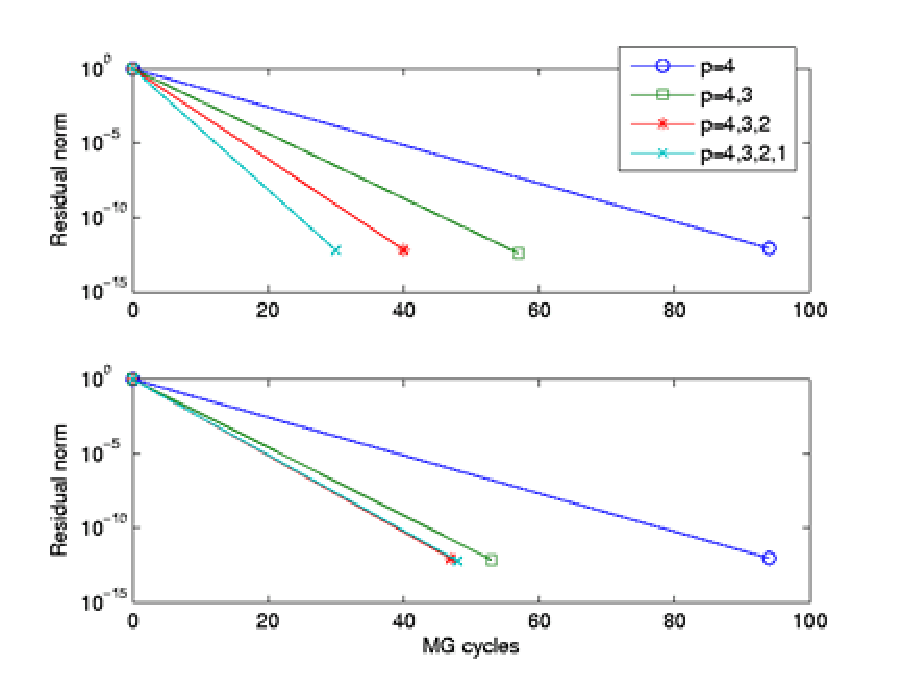
\includegraphics[width=90mm]{KimDfig1}
\end{center}

Figure 2 shows the accuracy versus CPU time:
\begin{center}
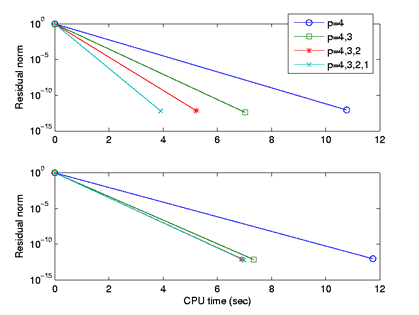
\includegraphics[width=90mm]{KimDfig2}
\end{center}


\begin{center}

\rule{6in}{1pt}
\end{center}

\begin{center}
{\large			\label{kimsd}
{\bf
A preconditioner on high-order finite element methods
}

Sang Dong Kim} \\
Department of Mathematics \\
Kyungpook National University \\
Taegu 702-701, Korea
\\ {\tt
skim@knu.ac.kr
}
\end{center}


Even if the high-order finite  element method has many advantages
for solving a uniformly self adjoint elliptic operator such as
\begin{equation*}
   Lu:= -\gradt\BA \nabla u  + c_0 u
   \quad \text{in}\quad \Omega=[-1,1]\times[-1,1]
\end{equation*}
with boundary conditions ( $\Gamma_L = \Gamma_D(L) \cup \Gamma_N(L))$
\begin{equation*}
   u=0 \quad \text{on} \quad \Gamma_D(L), \quad
   \bn \cdot\BA\nabla u = 0 \quad \text{on}\quad \Gamma_N(L),
\end{equation*}
one may have a difficulty controlling  condition numbers occurred
from spectral element discretizations which makes it uneasy to use
iterative methods. In order to alleviate such a situation, we take
a lower order finite element preconditioner operator corresponding
to
\begin{equation*}\label{pre:oper}
   Bv:= -\gradt \nabla u  + b_0 u
   \quad \text{in}\quad \Omega
\end{equation*}
with boundary conditions  ($\Gamma_B = \Gamma_D(B) \cup \Gamma_N(B))$
\begin{equation*}\label{pre:bdry}
   v=0 \quad \text{on} \quad \Gamma_D(B), \quad
   \bn \cdot\nabla v =0\quad \text{on}\quad
   \Gamma_N(B).
\end{equation*}
Let $\{ \eta_k\}^N_{k=0}$ be the standard Legendre-Gauss-Lobatto
(=:LGL) points in $[-1, 1]$.  By translations from $I$ to a
$j^{th}$ subinterval $I_j:=[x_{j-1},x_j]$ we denote
$\{\xi_k^j\}^N_{k=0}$ as the $k^{th}-$ LGL points in each
subinterval $I_j$ for $j= 1, 2, \cdots, M$. Let $\CP^h_N$ be the
subspace of $C[-1,1]$ which consists of piecewise polynomials
 with support $I_j=[x_{j-1}, x_j]$ whose degree is less
than or equal to $N$.  For the space $\CP^h_N$, we choose a {\it
piecewise Lagrange polynomial  basis functions} denoted as
$\{\phi^j_k(x)\}$ supported in $I_j$ for $ j=1, \cdots, M.$
Let ${\CV}_N^h$ be the space of all {\it piecewise Lagrange linear
functions} $\psi^i_k(x)$.  Define an interpolation operator
$\CI^h_N: C[-1, 1]\rightarrow \CP^h_N(I)$ such that
\begin{equation*}\label{int:INh}
  ( \CI_N^h v)(\xi_\mu) = v(\xi_\mu), \quad v\in C[-1, 1].
\end{equation*}
First, we set up  the following relations for $v\in {\CV}_N^h$
$$ c \|v\| \leq \| \CI_N^h v\| \leq C \|v\|, \quad
c \|v\|_1 \leq \| \CI_N^h v\|_1 \leq C \|v\|_1,$$
where two positive constants $c$ and $C$ do not independent of the
mesh size $h_j=x_j-x_{j-1}$ and the degree  $N$ of piecewise
polynomial. Let $(\hat{\mbox{\L}}_N^h)$ and $\hat{\BB}_N^h$ be   finite
element stiffness matrices corresponding to $L$ and $B$
respectively . Then  we will show the preconditioned system
$$ (\hat{\BB}_N^h)^{-1} \hat{L}_N^h$$
has positive  eigenvalues which are independent of the mesh size
$h_j=x_j-x_{j-1}$ and the degree $N$ of piecewise polynomial.


\begin{center}

\rule{6in}{1pt}
\end{center}

\begin{center}
{\large			\label{kimn}
{\bf
Implementation of An Overlapping Balancing Domain Decomposition Method
for Elliptic PDEs on Unstructured Meshes
}

Jung-Han Kimn} \\
Department of Mathematics and
The Center for Computation and Technology
\\
Louisiana State University
\\
Baton Rouge LA 70803
\\ {\tt
kimn@math.lsu.edu
}
\\
Blaise Bourdin
\end{center}

A new type of overlapping Domain Decomposition algorithm, Overlapping
Balancing Domain Decomposition (OBDD) algorithms, has been recently
presented by M. Sarkis and J.H. Kimn. This new algorithm can be
considered as an extension of the Balancing Domain Decomposition
algorithms to overlapping subdomains. This approach can be applied to
structured and unstructured meshes and relies on Partition of Unity
function to construct a sparse matrix for coarse space.

In this talk, we will discuss several aspects of the practical parallel
implementation of this method. We will show numerical results for large
unstructured meshes.

\begin{center}

\rule{6in}{1pt}
\end{center}

\begin{center}
{\large			\label{kolev}
{\bf
Experiments with Adaptive Element Agglomeration Algebraic Multigrid for
H(div) and H(curl).
}

Tzanio V. Kolev} \\
Center for Applied Scientific Computing \\
Lawrence Livermore National Laboratory \\
Box 808, L-560 \\ Livermore CA 94551
\\ {\tt
tzanio@llnl.gov
}
\\
Panayot S. Vassilevski
\end{center}

In this talk we combine the element agglomeration AMGe (from [2]) and
the adaptive AMG (from [1]). The former method is used to generate an
initial V-cycle that coarsens only the null space of the respective
H(div) or H(curl) form, whereas the second method is used to gradually
augment the current coarse grids and interpolation matrices. The
numerical tests indicate that 3 to 5 adaptive cycles are sufficient in
order to achieve an efficient AMG solver. A main tool in the adaptation
process is the hierarchical construction of the modified interpolation
matrices, see [3], which is based on solving local constrained
minimization problems, fitting one ``algebraically smooth'' vector at a
time.

[1] M.~Brezina, R.~Falgout, S.~MacLachlan, T.~Manteuffel, S.~McCormick,
and J.~Ruge, {\em Adaptive Algebraic Multigrid Methods},
SIAM J.~Sci.~Comp., 2004, submitted.

[2] J.~Jones and P.~Vassilevski, {\em AMGe Based on Element
Agglomerations}, SIAM J.~Sci.~Comp. {\bf 23} (2001), pp.109--133.

[3] P.~Vassilevski and L.~Zikatanov,
{\em Multiple Vector Preserving
Interpolation Mappings in Algebraic Multigrid},
Lawrence Livermore
National Laboratory Technical Report UCRL-JRNL-208036, November 2004.


\begin{center} \rule{6in}{1pt} \end{center}


\begin{center}
{\large			\label{lashuk}
{\bf Preconditioned eigensolvers in Hypre and PETSc}

Ilya Lashuk} \\
Department of Mathematics \\
University of Colorado \\
P.O. Box 173364, Campus Box 170 \\
Denver CO 80217-3364
\\ {\tt
ilashuk@math.cudenver.edu
}
\\
Merico Argentati,
Evgueni Ovtchinnikov,
Andrew Knyazev

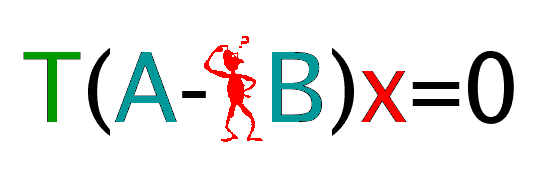
\includegraphics[width=60mm]{lashuk}
\end{center}

We present preliminary results of an ongoing project to develop codes
of the Locally Optimal Block Preconditioned Conjugate Gradient (LOBPCG)
method for symmetric eigenvalue problems for Hypre and PETSc software
packages. Hypre and PETSc packages provide high quality multigrid and
domain decomposition preconditioning on parallel clusters with
distributed or shared memory architecture. The LOBPCG method, suggested
and developed by Andrew Knyazev [1] in the past decade, recently
attracts an increasing attention as a potential alternative to the
shift-and-invert Lanczos and preconditioned Davidson methods due to its
simplicity robustness and fast convergence. Several MATLAB, C, C++ and
FORTRAN implementations of the LOBPCG are developed by different
groups, e. g., for such applications areas as structured mechanics and
electronic structure calculations. However, the only publicly available
at present LOBPCG implementation remains our implementation for Hypre,
which is already included in Hypre 1.8.2 release. We describe the
current state of the LOBPCG software for Hypre and PETSc, developed by
our group and demonstrate initial scalability results.

[1] A.V. Knyazev, {\em Toward the Optimal Preconditioned Eigensolver:
Locally Optimal Block Preconditioned Conjugate Gradient Method}.
SIAM Journal on Scientific Computing {\bf 23} (2001), 2, pp.517--541.


\begin{center} \rule{6in}{1pt} \end{center}
\newpage

\begin{center}
{\large			\label{lee}
{\bf
A Multilevel Time Parallelization Algorithm
}

Barry Lee} \\
LLNL, L-561 \\ P.O. Box 808 \\ Livermore CA 94550
\\ {\tt
lee123@llnl.gov
}
\\
Izaskun Garrido,
Gunnar E. Fladmark,
Magne S. Espedal
\end{center}

Parallel methods are usually not applied to the time domain because of
the inherit sequentialness of time evolution. But for many evolutionary
problems, computer simulation can benefit substantially from time
parallelization methods. In this talk, we present several such
multilevel algorithms that actually exploit the sequential nature of
time evolution through a predictor-corrector procedure. This
sequentialness ensures convergence of a parallel predictor corrector
procedure within a fixed number of iterations. The performance of these
novel algorithms which can be derived from the classical alternating
Schwarz method, are illustrated through several examples from reservoir
simulation.


\begin{center}

\rule{6in}{1pt}
\end{center}

\begin{center}
{\large			\label{limon}
{\bf
A Multilevel Adaptive Solver for the Density-Gradient Equation
}

Alfonso Limon} \\
School of Mathematical Sciences
\\
710 N. College Avenue
\\
Claremont CA 91711
\\ {\tt
alfonso.limon@cgu.edu
}
\\
Hedley Morris
\end{center}

Continuing advances in the miniaturization of integrated circuits have
imposed new challenges to designers of semiconductor devices, as
traditional circuit analysis tools are no longer applicable. In this
study, we focus on the gate region of MOSFET devices with an oxide
thickness of order 4-6 nanometers. For oxide layers of this width,
quantum effects start to become noticeable and the standard equations
of semiconductor physics require quantum corrections. The
Density-Gradient equation [1], [2] is a means of calculating
approximate quantum corrections to existing formulae without solving
the full Poisson-Schr\"{o}dinger system.

We use a one-dimensional
approximation to reduce the D-G equations to a set of singularly
perturbed ODEs [3]. These equations have interior layer solutions,
which compromise the numerical treatment of the problem if care is not
taken to resolve the large gradients in the solution within the layer
correctly. Several approaches have been proposed to resolve the
boundary layer region including nonlinear discretization schemes [4],
[5]. However, these methods have difficulty resolving interior layers
[6]; therefore, we propose a multilevel adaptive scheme to solve the
model equations. The method is akin to multigrid, but utilizes
high-order inter-grid operators, which preserve a nested space
structure throughout the various resolution levels, similar to the
methods described by Goedecker [7] and Warming \& Beam [8]. This
multilevel method has several advantages over the previous
discretization schemes, the most important being that it adapts
dynamically to interior layers without a priori knowledge of the
location or geometry of the layer.

[1] Ancona M.G. 1990.
{\em Macroscopic description of quantum-mechanical tunneling}.
Phys.~Rev.~B {\bf 42}: 1222.

[2] Ancona M.G. 1998.
{\em Simulation of quantum confinement effects in
Ultra-Thin-oxide MOS structures}. J.~Tech.~CAD (11).

[3] Ward, J. F., Odeh M., and Cohen D. S.,
{\em Asymptotic methods for metal
oxide semiconductor field affect transistor modeling}.
SIAM J.~Appl.~Math {\bf 50} 1099--1125 (1990).

[4] Ancona M.G. and Biegel B.A. 2000.
{\em Nonlinear discretization scheme
for the density-gradient equations}. In Proc. SISPAD~R00, p.196
(2000).

[5] Wettstein A., Schenk A., and Fichtner W. 2001.
{\em Quantum device-simulation with the density-gradient model
on unstructured grids}. IEEE Trans. Elec. Dev. 48: 279.

[6] Wang X. and Tang T.-W. 2002.
{\em Discretization scheme for Density-Gradient Equation}.
Journal of Computational Electronics 1,
389-392.

[7] Goedecker S., Ivanov O., {\em Solution of Partial Differential
Equations Using Wavelets}, Comp. In Phys, 12, 548 (1998) .

[8] Warming R., Beam R, {\em Discrete Multiresolution Analysis Using
Hermite Interpolating: Biorthogonal Multiwavelets}, SIAM J. Sci.
Comput. 22, 4, 1269-1377 (2000).

\begin{center}

\rule{6in}{1pt}
\end{center}

\begin{center}
{\large			\label{livshits}
{\bf
Multilevel eigenbasis for Schr\"{o}dinger eigenvalue problems
}

Irene Livshits} \\
Department of Mathematical Sciences \\
Ball State University \\
Muncie IN 47306
\\ {\tt
ilivshits@bsu.edu
}
\end{center}

In this talk we discuss AMG algorithms for eigenbasis approximation for
Schr\"{o}dinger eigenvalue problems with variable potential. The algorithms
employ the multilevel eigenvalue structure suggested by Livne and
Brandt, and are used to solve one-dimensional
(at $O(N\log N)$ operations)
and two-dimensional problems (at somewhat comparable costs). Also to be
addressed is the issue of the quality of the approximated eigenbasis,
such as its fullness and independence of the eigenfunctions. Numerical
results for both one- and two-dimensional problems will be discussed.

\begin{center}

\rule{6in}{1pt}
\end{center}

\begin{center}
{\large			\label{maclachlan}
{\bf
Fully Adaptive AMG
}

Scott MacLachlan} \\
Department of Applied Mathematics \\
University of Colorado \\
Boulder CO 80309-0526
\\ {\tt
maclachl@colorado.edu
}
\end{center}

Numerical simulation of physical processes is often constrained by our
ability to solve the complex linear systems at the core of the
computation. Classical geometric and algebraic multigrid methods rely
on (implicit) assumptions about the character of these matrices in
order to develop appropriately complementary coarse-grid correction
processes for a given relaxation scheme. The aim of the adaptive
multigrid framework is to reduce the restrictions imposed by such
assumptions, thus allowing for efficient black-box multigrid solution
of a wider class of problems.

There are, however, many challenges in altogether removing the reliance
on assumptions about the errors left after relaxation. In this talk, we
discuss work to date on a fully adaptive AMG algorithm that chooses all
components of the coarse-grid correction based on automated analysis of
the performance of relaxation. Fundamental measures of the need for and
quality of a coarse-grid correction will be discussed, along with
related techniques for choosing coarse grids and interpolation
operators. We will also discuss the (lack of) computability of these
ideal measures, and suggest cost-efficient alternatives.

This research has been performed in collaboration with James Brannick,
Marian Brezina, Tom Manteuffel, Steve McCormick, and John Ruge at
CU-Boulder. It has been supported by an NSF SciDAC grant (TOPS), as
well as Lawrence Livermore and Los Alamos National Laboratories.

\begin{center}

\rule{6in}{1pt}
\end{center}

\begin{center}
{\large			\label{masson}
{\bf
Block Preconditioners with Algebraic Multigrid Block Solve in
Stratigraphic Modeling for oil exploration
}

Roland Masson} \\
Institut Francais du Petrole \\
1 et 4 Avenue Bois Preau, 92000 Rueil \\
Malmaison, France
\\ {\tt
roland.masson@ifp.fr
}
\\
V\'{e}ronique Gervais
\end{center}

Stratigraphic models simulate the erosion and sedimentation of
sedimentary basins at geological time scales given the sea level
variations, the tectonics displacements of the basement, and the
sediments fluxes at the boundary of the basin. We consider in this talk
a sediments transport model coupling three main processes: a gravity
driven transport of the sediments for which the fluxes are proportional
to the gradient of the topography, a weather limited transport taking
into account the disymmetry between erosion and sedimentation, and a
fluvial transport model for which the sediments fluxes are proportional
to the water discharge. The main variables of the problem are the
sediment thickness, a flux limitor, and the $L$ sediments concentrations
in basic lithologies such as sand or shale or carbonates. Such model is
applied in oil exploration for a better prediction of potential
reservoirs location. The model is derived writing the mass conservation
of each lithology leading to a system of mixed parabolic hyperbolic
type. It is discretized by a finite volume scheme in space and a fully
implicit time integration, leading to the solution at each time step of
a non linear systems of $L+2$ variables on the 2D mesh.

After Newton type
linearization, we are left with the solution of an ill conditioned
linear system with sharp jumps in the diffusion coefficients and
coupling $L+2$ variables of mixed types. These linear systems are solved
using an iterative solver and a block approach for the preconditioner
in order to separate the different variables. In a first step, a
mixture equation is obtained by linear combinations of the rows that
should concentrate the ellipticity of the system and as much as
possible decouple the first two variables (sediment thickness and flux
limitor) from the $L$ concentrations variables. Then the overall system
is solved using a block Gauss Seidel preconditioner. The First block
(sediment thickness and flux limitor variables) is preconditioned
either by a direct sparse solver or by an ILU0 incomplete
factorization, or by a vcycle of an algebraic multigrid solver (AMG1R5
from Ruge and Stueben) on the sediment thickness sub-block only in order
to avoid non diagonal dominance. The remaining blocks are solve using a
gauss seidel sweep in topographical order leading to an exact inversion
of these blocks. These block preconditioners are compared with a sparse
direct solver and an ILU0 incomplete factorization on the overall
system. The comparison is made in terms of CPU time, and scalability
with respect to the mesh size and the jump of the diffusion
coefficients on two real test cases: the Paris basin and a Rift test
case with water discharge. It shows that the block approach combined
with a multigrid preconditioning of the the sediment thickness
sub-block is a very efficient method, nearly scalable for this problem.


\begin{center} \rule{6in}{1pt} \end{center}
\newpage	% H


\begin{center}
{\large			\label{mavriplis}
{\bf
Multigrid solution of the lattice Boltzmann equation
}

Dimitri J. Mavriplis} \\ 
Department of Mechanical Engineering \\
University of Wyoming \\
Laramie WY 82071
\\ {\tt
mavripl@uwyo.edu
}
\end{center}

The last decade has seen rapid progress in the theoretical
understanding, algorithmic development, and use of lattice Boltzmann
methods (LBM). As opposed to traditional computational fluid dynamics
approaches, which compute macroscopic fluid dynamic properties by
discretizing the continuum governing equations, the independent
variables in a lattice Boltzmann approach consist of particle
distribution functions in phase space, from which macroscopic continuum
fluid properties can be recovered. Historically, LBM methods have been
derived from lattice gas automata (LGA) methods. LGA methods model
macroscopic fluid motion through the evolution of a set of discrete
particles on a regular lattice (cartesian grid). Many of the
deficiencies of LGA methods in reproducing accurate macroscopic
behavior were resolved by the LBM approach, by neglecting individual
particle motion, and adopting a particle distribution function
approach. However, LBM methods have retained this conceptual link to
particle methods such as LGA, which has inhibited the use of more
sophisticated numerical techniques.

In this work, we first describe the lattice Boltzmann method as a
particular finite-difference discretization in space and time of the
Boltzmann equation. The LBM time-step is then shown to be equivalent to
a first-order explicit time step (forward Euler), which is also
equivalent to a Jacobi iteration for the steady-state form of the LBM
equations. It is then shown how this iteration strategy may be used as
a solver for the steady-state lattice Boltzmann equation, or as a
solver for an implicit time-integration strategy. Finally, it is shown
how these problems may be solved more efficiently using the Jacobi
iteration as a smoother in a multigrid scheme for the steady-state
lattice Boltzmann equation. This requires under-relaxation of the
iteration scheme to achieve good high-frequency damping properties, and
a careful matching of the LBM discretizations on the coarse grid
levels, in order to ensure consistent coarse and fine grid problems.
The final result is a multigrid solver which can make use of a
pre-existing LBM routine in a modular fashion, by invoking the LBM
routine on each grid level. Convergence rates which are independent of
the mesh resolution are demonstrated for the driven cavity problem on a
cartesian grid, although the convergence rates degrade with increasing
Reynolds number.

[1] D.~J.~Mavriplis, {\em Multigrid Solution of the Steady-State Lattice
Boltzmann Equation}, paper delivered at International Conference for
Mesoscopic Methods in Engineering and Science (ICMMES), Braunschweig,
Germany, July 2004. To appear in Computers and Fluids, 2005.


\begin{center} \rule{6in}{1pt} \end{center}
\newpage	% H


\begin{center}
{\large			\label{mehl}
{\bf
A cache-oblivious self-adaptive full multigrid method
}

Miriam Mehl} \\
Institut f\"{u}r Informatik, TU M\"{u}nchen \\
Boltzmannstr. 3 \\
85748 Garching, Germany
\\ {\tt
mehl@in.tum.de
}
\\
Nadine Dieminger,
Christoph Zenger
\end{center}

In many implementations of modern solvers for partial differential
equations, the use of multigrid methods in particular in combination
with dynamically adaptive grids causes a non-negligible loss of
efficiency in data access and storage usage: As multilevel data on
adaptively refined grids are typically organized in trees and stored
with the help of pointer structures, the evaluation of difference
stencils, restrictions and interpolations generate jumps within the
physical memory space and, thus, prevent an efficient usage of
cache-hierarchies and prefetching strategies. In addition, the storage
of pointers to neighbors, fathers and sons of each grid cell is
required. Our algorithm overcomes these inefficiencies by a
linearization of all data with the help of space-trees and
space-filling curves. Space-filling curves are well known as an
efficient tool for parallelization strategies on space-tree grids as
they define a linear ordering of all grid cells and, thus, allow a
simple partitioning of data. Space-tree grids are structured grids but,
at the same time, permit arbitrary local refinement (The only exception
are unisotropic refinements. The realization of such refinements is
subject of our current studies.).

In our algorithm, we associate the degrees of freedom of the unknown
function(s) to the vertices of the grid cells and - as a first step
towards cache-optimality - we replace the common pointwise operator
evaluation - that is the complete computation of the operator value at
a grid point necessitating access to data of neighboring points and,
thus, causing a part of the jumps within the physical memory space. We
use an elementwise operator evaluation instead: We decompose the
pointwise difference stencils in parts only incorporating vertex data
of the actual cell and get the overall operator value by accumulation
over all cells involved. From the algorithmic point of view, the
consequence is a cellwise instead of pointwise processing of the
space-tree grid during the iterations of our solver.

The second and crucial step on our way to cache-optimality is to
construct suitable data structures with minimal storage overhead and
strictly local access properties. If we use the discrete iterates of
the Peano-curve, a self-similar recursively defined space-filling
curve, to define a top-down-depth-first processing order of the grid
cells (on all levels), we can derive a storage concept with a fixed,
small and constant number of stacks as the only kind of data structures
[1,2,3,4]: Due to the dimension-recursivity of the Peano-curve, this
traversal order leads to a to-and-fro-processing of vertex data on
certain sub-manifolds of the domain which exactly fits the properties
of stacks: Stacks are very simple data structures allowing only the two
basic operations push and pop (push puts data on top of a pile and pop
takes data from the top of a pile). Due to this, the locality of data
access is inherently very high which makes data access very fast - even
faster than the common access of non-hierarchical data stored in
matrices - and, in particular, reduces cache misses considerably. In
addition, we can define locally deterministic rules for pushing and
poping data to/from the set of stacks. Thus, also the storage overhead
for administrational information is minimal. Each cell only has to
carry one bit for geometrical and one bit for refinement information.

Dynamical adaptivity can be realized in a very natural way in this
concept by definition of data sources and sinks at interface to the
input and output stacks of a solver iteration. Based on the algorithmic
concepts described above, we implemented an adaptive Full Multigrid
method for the three-dimensional Poisson equation with several
adaptivity criteria like shape of the domain, error estimators for the
global error and dual approaches to handle local accuracy requirements.
In addition, the Multigrid method was combined with a tau-extrapolation
scheme to achieve a fourth order discretization [5,6]. Thus, we
considerably enhanced the numerical efficiency without loosing
cache-efficiency compared to a simple non-adaptive one-level solver. In
all case studies, the number of actual cache misses is only about ten
percent higher than the unavoidable minimum of cache misses caused by
the first loading of data points to the cache.

[1] F.~G\"{u}nther, M.~Mehl, M.~P\"{o}gl, Ch.~Zenger,
{\em A cache-aware
algorithm for PDEs on hierarchical data structures},
Conference Proceedings PARA '04, Kopenhagen, June 2004,
LNCS, Springer, submitted.F.

[2] F.~G\"{u}nther, M.~Mehl, M.~P\"{o}gl, Ch.~Zenger,
{\em A cache-aware
algorithm for PDEs on hierarchical data structures based on
space-filling curves}, SIAM Journal on Scientific Computing,
in review.

[3] F.~G\"{u}nther,
{\em A Cache-Optimal Implementation of the
Finite-Element-Method} (German: Eine cache-optimale
Implementierung der Finite-Elemente-Methode), Doctoral
Thesis, Institut f\"{u}r Informatik, TU M\"{u}nchen, 2004.

[4] M.~P\"{o}gl,
{\em Development of a Cache-Optimal 3D
Finite-Element-Method for Big Problems} (German:
Entwicklung eines cache-optimalen 3D
Finite-Element-Verfahrens f\"{u}r groe Probleme),
Doctoral Thesis, Institut f\"{u}r Informatik, TU
M\"{u}nchen, 2004.

[5] A.~Krahnke,
{\em Adaptive Higher Order Methods on Cache-Optimal
Datastructures for Three-Dimensional Problems} (German:
Adaptive Verfahren hherer Ordnung auf cache-optimalen
Datenstrukturen f\"{u}r dreidimensionale Probleme),
Doctoral Thesis, Institut f\"{u}r Informatik, TU
M\"{u}nchen, 2005.

[6] N.~Dieminger,
{\em Criteria for the Selfadaption of
Cache-Efficient Multigrid Algorithms} (German: Kriterien
f\"{u}r die Selbstadaption cache-effizienter
Mehrgitteralgorithmen), Diploma Thesis, Institut f\"{u}r
Informatik, TU M\"{u}nchen, 2005.


\begin{center}

\rule{6in}{1pt}
\end{center}

\begin{center}
{\large			\label{meir}
{\bf
The Action-Dependent Wave Function Problem: Well Posedness and
Efficient Numerical Solutions
}

A. J. Meir} \\
Department of Mathematics and Statistics \\
232 Parker Hall \\
Auburn University \\
Auburn AL 36830

Irad Yavneh
\end{center}


We describe some results for a mixed (elliptic-hyperbolic) partial
differential equation and an efficient multigrid algorithm for its
numerical solution. The problem models an equation which arises in
atomic physics and describes a new object: an ``action-dependent wave
function.''



\begin{center}

\rule{6in}{1pt}
\end{center}

\begin{center}
{\large			\label{moulton}
{\bf
Multilevel Upscaling: Multigrid's Lost Twin
}

J. David Moulton} \\
MS B284 \\
Los Alamos National Laboratory \\
Los Alamos NM 87545
\\ {\tt
moulton@lanl.gov
}
\\
Scott P. MacLachlan
\end{center}

In many applications, homogenization (or upscaling) techniques are
necessary to develop computationally feasible models on scales coarser
than the variation of the coefficients of the continuum model. The
accuracy of such techniques depends dramatically on assumptions that
underlie the particular upscaling methodology used. For example,
decoupling of fine- and coarse-scale effects in the underlying medium
may utilize artificial internal boundary conditions on sub-cell
problems. Such assumptions, however, may be at odds with the true,
fine-scale solution, yielding coarse-scale errors that may be
unbounded.

In this work, we present an efficient multilevel upscaling (MLUPS)
procedure for single-phase saturated flow through porous media.
Coarse-scale models are explicitly created from a given fine-scale
model through the application of standard operator-induced variational
coarsening techniques. Such coarsenings, which originated with robust
multigrid solvers, have been shown to accurately capture the influence
of fine-scale heterogeneity over the complete hierarchy of resulting
coarse-scale models. Moreover, implicit in this hierarchy is the
construction of interpolation operators that provide a natural and
complete multiscale basis for the fine-scale problem. Thus, this new
multilevel upscaling methodology is similar to the Multiscale Finite
Element Method (MSFEM) and, indeed, we show that it attains similar
accuracy on a variety of problems. While MSFEM is based on a two-scale
approach, MLUPS generates a complete hierarchy of coarse-scale models,
resulting in a speed-up factor of approximately 15. In addition, we
demonstrate that this new upscaling methodology can use both structured
coarsening algorithms, such as Dendy's BoxMG, and fully algebraic
algorithms, such as Ruge's AMG.

\begin{center}

\rule{6in}{1pt}
\end{center}

\begin{center}
{\large			\label{nastase}
{\bf
High-Order Spectral $hp$-Multigrid Methods on Unstructured Grids
}

Cristian R. Nastase} \\
Department of Mechanical Engineering \\
University of Wyoming \\
1000 E. University Ave. \\
Laramie WY 82071-3295
\\ {\tt
nastase@uwyo.edu
}
\\
Dimitri J. Mavriplis
\end{center}

The development of optimal, or near optimal solution strategies for
higher-order discretizations, including steady-state solutions
methodologies, and implicit time integration strategies, remains one of
the key determining factors in devising higher-order methods which are
not just competitive but superior to lower-order methods in overall
accuracy and efficiency. The goal of this work is to investigate and
develop a fast and robust algorithm for the solution of high-order
accurate Discontinuous Galerkin discretizations of non-linear systems
of conservation laws on unstructured grids. Herein we extend the
spectral multigrid approach described in [1] to the two-dimensional
steady-state Euler equations, and couple the spectral $p$-multigrid
approach with a more traditional agglomeration $h$-multigrid method for
unstructured meshes. The investigation of efficient smoothers to be
used at each level of the multigrid algorithm is also pursued, and
comparisons between linear and non-linear solver strategies are made as
well [2]. The overall goal is the development of a solution algorithm
which delivers convergence rates which are independent of ``$p$" (the
order of accuracy of the discretization) and independent of ``$h$" (the
degree of mesh resolution), while minimizing the cost of each
iteration.

The computational domain is partitioned into an ensemble of
non-overlapping unstructured elements and within each element the
solution is approximated by a truncated polynomial expansion. The
semi-discrete formulation employs a local discontinuous Galerkin
formulation in spatial variables within each element. Thus, the
solution approximation is local, discontinuous, and doubled valued on
each elemental interface. Monotone numerical fluxes are used to resolve
the discontinuity, providing the means of communication between
adjacent elements and specification of the boundary conditions. An
approximate Riemann solver is used to compute the flux at inter-element
boundaries. The discrete form of the local discontinuous Galerkin
formulation is defined by the particular choice of the set of basis
functions. Hereby a set of hierarchical basis functions is used in
order to simplify our subsequent spectral multigrid implementation. The
full description of the basis function set is given in [3]. The
resulting set of equations is solved in the modal space and the
integrals are evaluated by Gaussian quadrature rules.

The spectral $p$-multigrid approach is based on the same concepts as a
traditional $h$-multigrid method, but makes use of ``coarser'' levels
which are constructed by reducing the order of accuracy of the
discretization, rather than using physically coarser grids with fewer
elements. Furthermore, the formulation of the interpolation operators,
between fine and coarse grid levels, is greatly simplified when a
hierarchical basis set is employed for the solution approximation. The
main advantage is due to the fact that the lower order basis functions
are a subset of the higher order basis (i.e. hierarchical) and the
restriction and prolongation operators become simple projection
operators into a lower and higher order space, respectively [4]. For
pure $p$-multigrid methods, the recursive application of lower order
discretizations ends with the $p=0$ discretization on the same grid as
the fine level problem. For relatively fine meshes, the (exact)
solution of this $p=0$ problem at each multigrid cycle can become
expensive, and may impede the $h$-independence property of the multigrid
strategy. The $p=0$ problem can either be solved approximately by
employing the same number of smoothing cycles on this level as on the
finer $p$-levels, or it can be solved more accurately by performing a
larger number of smoothing cycles at each visit to this coarsest level.
In either case, the convergence efficiency will be compromised, either
due to inadequate coarse level convergence, or due to excessive coarse
level solution cost. An alternative is to employ an $h$-multigrid
procedure to solve the coarse level problem at each multigrid cycle. In
this scenario, the $p$-multigrid scheme reverts to an agglomeration
multigrid scheme once the $p=0$ level has been reached, making use of a
complete sequence of physically coarser agglomerated grids, thus the
designation $hp$-multigrid. First-order accurate (p=0) agglomeration
multigrid methods for unstructured meshes are well established [5] and
deliver near optimal convergence rates. Therefore, this procedure has
the potential of resulting in a truly $h$- and $p$-independent solution
strategy for high-order accurate discontinuous Galerkin
discretizations.

At each $h$- or $p$-multigrid level an element-Jacobi type scheme is used
as a smoother. The element-Jacobi scheme can be viewed as an
approximate Newton scheme where the full Jacobian matrix is replaced by
the block diagonal entries representing the coupling between all modes
within each element, [D], thus neglecting the coupling between
neighboring element modes, which arises through the inter-element flux
evaluations. The [D] blocks represent small dense matrices associated
with each grid element. A second variant of this solver is denoted as
the ``linearized" element-Jacobi method. In this approach, the full
Jacobian matrix is retained, but is decomposed into block diagonal [D]
and off-diagonal [O] components. Note that the linearized element
Jacobi scheme involves a dual iteration strategy, where each nth outer
non-linear iteration entails ``k" inner linear iterations. The
advantage of this formulation is that the non-linear residual and the
Jacobian entries, [D] and [O], are held constant during the linear
iterations. This can significantly reduce the required computational
time per cycle for expensive non-linear residual constructions. Because
this scheme represents an exact linearization of the element-Jacobi
scheme both approaches can be expected to converge asymptotically at
the same rates per cycle [6]. The convergence can be further
accelerated by using a Gauss-Seidel strategy where the off-diagonal
matrices are split into lower, [L], and upper, [U] contributions (i.e.
[O]=[L]+[U]). This last solver variant, again, involves a dual
iteration strategy, but follows an ordered sweep across the elements
using latest available neighboring information in the Gauss-Seidel
sense. In this work, we employ a frontal sweep along the elements which
begins near the inner boundary and proceeds toward the outer boundary,
using the numbering assigned to the grid elements from an advancing
front mesh generation technique.

The resulting $hp$-multigrid scheme demonstrates $p$-independent and nearly
$h$-independent convergence rates. The coupling of $p$- and $h$-multigrid
procedures, through the use of agglomerated coarse levels for
unstructured meshes, increases the overall solution efficiency compared
to a $p$-alone multigrid procedure, and the benefits of the $hp$-multigrid
approach can be expected to increase for finer meshes. The multigrid
procedure can itself be applied as a non-linear solver (FAS), or as a
linear solver (CGC) for a Newton scheme applied to the non-linear
problem. The linear multigrid approach demonstrates superior overall
efficiency, provided a suitable linear iteration termination strategy
is employed. Results are presented for compressible flow over a bump in
a channel and for flow over a four element airfoil in two dimensions.


[1] Helenbrook, B. and Mavriplis, D. J. and Atkins, H.,
{\em Analysis of
``p''-Multigrid for Continuous and Discontinuous Finite Element
Discretizations}, Proceedings of the 16th AIAA Computational Fluid
Dynamics Conference, 2003, AIAA Paper 2003-3989.

[2] Nastase, C.R. and Mavriplis, D.J.,
{\em High-Order Discontinuous
Galerkin Methods using a Spectral Multigrid Approach}, Proceedings of
the 43rd AIAA Aerospace Sciences Meeting and Exhibit, 2005, AIAA Paper
2005-1268.

[3] Solin, P. and Segeth, P. and Zel, I.D.,
{\em High-Order Finite Element Methods}, Chapman and Hall, 2003.

[4] Fidkowski, K.J. and Darmofal, D.L.,
{\em Development of a
Higher-Order Solver for Aerodynamic Applications}, Proceedings of the
42nd AIAA Aerospace Sciences Meeting and Exhibit, 2004, AIAA Paper
2004-0436.

[5] Mavriplis, D. J. and Venkatakrishnan, V.,
{\em Agglomeration Multigrid for Two Dimensional Viscous Flows},
Computers and Fluids, 24(5):553--570, 1995.

[6] Mavriplis, D.J.,
{\em An Assessment of Linear versus Non-Linear
Multigrid Methods for Unstructured Mesh Solvers},
J.~Comput.~Phys., 175:302--325, 2002.

\begin{center}

\rule{6in}{1pt}
\end{center}

\begin{center}
{\large			\label{niet}
{\bf
Multilevel Preconditioners in Thermohaline Ocean Circulation
}

Arie de Niet} \\
Research Institute for Mathematics and Computing Science
\\
University of Groningen
\\
P.O.Box 800 \\
9700 AV Groningen \\
The Netherlands
\\ {\tt
a.c.de.niet@math.rug.nl
}
\\
Fred Wubs
\end{center}

The numerical continuation of steady states in thermohaline ocean
circulation requires the solution of large systems. The (linearized)
equations describing the thermohaline ocean circulation (for a detailed
description of these equations see [5]) can be split into equations
for velocities in longitudinal and latitudinal direction ($x_{uv}$),
velocity in vertical direction ($x_w$), pressure ($x_p$) and salinity and
temperature ($x_{ST}$). The equations are coupled in the following way,
$$ \left( \begin{array}{cccc}
A_{uv} & 0 & G_{uv} & 0 \\
0 & 0 & G_w & B_{ST} \\
D_{uv} & D_w & 0 & 0 \\
B_{uv} & B_w & 0 & A_{ST}
\end{array}\right)
\left( \begin{array}{c}
	x_{uv} \\ x_{w} \\ x_{p} \\ x_{ST}
	\end{array}\right)
= \left( \begin{array}{c}
	b_{uv} \\ b_{w} \\ b_{p} \\ b_{ST}
	\end{array}\right)
$$
where $G*$ represents the discrete gradient operator and $D*$ the discrete
divergence operator. We assume that $G*T=D*$, i.e. the discrete operators
are each others transpose. Furthermore, $A_{ST}$ is a convection-diffusion
matrix, $A_{uv}$ is also a convection-diffusion matrix, but includes a
Coriolis force. Respectively the four equations describe conservation
of momentum (in longitudinal and latitudinal direction), the
hydrostatic pressure, conservation of mass and conservation of salt and
heat.

Due to the size of the systems they are solved via a Krylov subspace
method using a preconditioner to speed up the convergence. In general
there are two ways to obtain a preconditioner for the matrix in the
equation. One could try to exploit the structure of the system or apply
a general black-box preconditioning method like an incomplete LU
factorization. We will do both and compare the results.

In the current code for numerical simulation of thermohaline ocean
circulation (THCM, see [5], the systems are solved with the MRILU [1]
preconditioner. MRILU is a multilevel ILU method containing ideas
similar to algebraic multigrid methods. However MRILU doesn't need any
smoothing steps, because of sophisticated dropping- and lumping
criteria. In THCM MRILU is applied to the clustered equations, that is
the six unknowns ($u$,$v$,$w$,$p$,$T$,$S$),
that belong to one and the same cell,
are treated as one unknown. The method is able to construct a good
factorization and the Krylov subspace method converges fast.
Unfortunately the preconditioner requires a lot of construction time
and memory, which becomes a problem if the size of the problem is
increased.

In order to reduce the memory usage, we developed an alternative
preconditioner that exploits the structure. The ingredients are: a
splitting of the pressure in a depth-averaged pressure and a component
perpendicular to that; a non-symmetric reordering of the matrix;
dropping the block $B_{ST}$. This together gives a block-Gauss-Seidel
preconditioner, that requires some matrix-vector products and the
solution of three relatively easy systems: (i) a depth-averaged saddle
point system based on $A_{uv}$, $G_{uv}$ and $D_{uv}$, (ii) a
convection-diffusion-Coriolis equation involving $A_{uv}$ and (iii) a
convection-diffusion equation involving $A_{ST}$. The last two problems can
be handled very well by MRILU. For the saddle point system we can apply
any of the preconditioners from literature [3,4] or the ones we
developed ourselves based on artificial compressibility and
grad-div-stabilization [2] respectively.

A comparison of the structured preconditioner with MRILU applied to the
subsystems and MRILU applied to the clustered matrix at once shows that
the required amount of memory is reduced with almost a factor 10. We
have to pay for that in an increase of the number of iterations in the
Krylov subspace method, but this factor is at most 2. Overall we see a
serious speed up.

On the conference we will describe the block-Gauss-Seidel
preconditioner and show the results of a comparison using both MRILU
and an algebraic multigrid method as a subsolver in the preconditioner.

[1]
E. F. F. Botta and F. W. Wubs.
{\em Matrix renumbering ILU: an effective algebraic multilevel ILU
preconditioner for sparse matrices}.
SIAM J.~Matrix~Anal.~Appl., {\bf 20(4)}:1007--1026 (electronic),
1999.
Sparse and structured matrices and their applications
(Coeur d'Alene, ID, 1996).

[2]
Arie C. de Niet and Fred W. Wubs.
{\em Two preconditioners for the saddle point
equation}.
In Proceedings of the European Congres on
Computational Methods in Applied Sciences
and Engineering (ECCOMAS,
Jyv\"{a}skyl\"{a}, 2004).
See http://www.mit.jyu.fi/eccomas2004/.

[3]
Howard C. Elman, David J.
Silvester, and Andrew J. Wathen.
{\em Performance and analysis of
saddle point preconditioners
for the discrete steady-state
Navier-Stokes equations}.
Numer. Math., {\bf 90(4)}:665a--688, 2002.

[4]
C. Vuik and A. Saghir.
{\em The Krylov accelerated SIMPLE(R) method for incompressible flow}.
Report 02-01, Delft University of Technology, Department of Applied
Mathematical Analysis, Delft, 2002.

[5]
Weijer Wilbert, Henk A.  Dijkstra, Hakan Oksuzoglu, Fred W.  Wubs, and
Arie C. de Niet.
{\em A fully-implicit model of the global ocean circulation}.
J.~Comp.~Phys., {\bf 192}:452--470, 2003.


\begin{center} \rule{6in}{1pt} \end{center}


\begin{center}
{\large			\label{nishida}
{\bf
AMG Preconditioned Conjugate Gradient Type Methods
for Nonsymmetric Eigenproblems
}

Akira Nishida} \\
Department of Computer Science, Univerisity of Tokyo \\
7-3-1, Hongo, Bunkyo-ku, Tokyo \\
113-0033 JAPAN
\\ {\tt
nishida@is.s.u-tokyo.ac.jp
}
\end{center}


When we need to compute the eigenvalues of a large sparse matrix
numerically, the projection method such as the Lanczos type or the
Davidson type methods has been the most orthodox choice. However,
recent studies revealed that the conjugate gradient method combined
with appropriate preconditioners can compute a few eigenpairs of such
problems quite efficiently. For large scale nonsymmetric eigenproblems,
we expand this approach to the conjugate residual and the bi-conjugate
gradient type methods, and evaluate the combination with the AMG
preconditioner.


\begin{center} \rule{6in}{1pt} \end{center}
\newpage	% HEY


\begin{center}
{\large			\label{olson}
{\bf
Algebraic Multigrid (AMG) for Higher-Order Finite Elements
}

Luke Olson} \\
Division of Applied Mathematics \\
Brown University
\\ {\tt
lolson@dam.brown.edu
}
\\
Jeff Heys,
Tom Manteuffel,
Steve McCormick
\end{center}


In this talk we consider two related approaches for solving linear
systems that arise from a higher-order finite element discretization of
elliptic partial differential equations. The first approach explores
direct application of an algebraic-based multigrid method (AMG) to
iteratively solve the linear systems that result from higher-order
discretizations. While the choice of basis used on the discretization
has a significant impact on the performance of the solver, results
indicate that AMG is capable of solving operators from both Poisson's
equation and a first-order system least-squares (FOSLS) formulation of
Stoke's equation in a scalable manner, nearly independent of basis
order, $p$. The second approach incorporates preconditioning based on a
bilinear finite element mesh overlaying the entire set of degrees of
freedom in the higher-order scheme. AMG is applied to the operator
based on the bilinear finite element discretization and is used as a
preconditioner in a conjugate gradient (CG) iteration to solve the
algebraic system derived from the high-order discretization. This
approach is also nearly independent of $p$. We present several numerical
examples that support each method and discuss the computational
advantages of the preconditioning implementation.

\begin{center}

\rule{6in}{1pt}
\end{center}

\begin{center}
{\large			\label{oosterlee}
{\bf
Multigrid for a segregated version of the poroelasticity system
}

Cornelis W. Oosterlee} \\
Delft University of Technology, DIAM \\
Mekelweg 4, 2628 CD Delft \\
the Netherlands
\\ {\tt
c.w.oosterlee@ewi.tudelft.nl
}
\\
Fransisco J. Gaspar,  Francisco J. Lisbona
\end{center}

Poroelasticity has a wide range of applications in biology, filtration,
tissue engineering and soil sciences. It represents a model for
problems where an elastic porous solid is saturated by a viscous fluid.
The poroelasticity equations were derived by Biot in 1941, studying the
consolidation of soils. In this talk we will present an efficient
solution method for the poroelasticity system. A staggered grid
discretization is adopted from incompressible flow and modified for the
poroelasticity system. Standard finite elements (or finite differences)
do not lead to stable solutions without additional stabilization. The
staggered grid discretization leads to a natural stable discretization.
In contrast to our previous work, where we provided multigrid
solvers for the whole system of poroelasticity equations, here we first
split the system into scalar equations. This splitting can be
interpreted as a segregated solution approach, similarly to
pressure-correction methods in incompressible fluid flow simulation. In
fact, we just reverse loops as compared to our previous work: The
distributive smoothing method from now acts as the "outer loop" in
the solution process. The method can also be seen as a form of
preconditioning of the original poroelasticity system. Next to a right-
we also present the left-preconditioned system and corresponding
results. In the segregated framework we need to solve for scalar
equations only, thus enabling the solution of three-dimensional
problems on relatively fine grids. Highly efficient multigrid schemes
are used to solve the resulting scalar equations. Next to numerical
experiments and analysis results we will present some theoretical
convergence results for the approach adopted.

\begin{center}

\rule{6in}{1pt}
\end{center}

\begin{center}
{\large			\label{ovtchinnikov}
{\bf
A Fully Coupled Implicit Method for A Magnetohydrodynamics Problem
}

Serguei Ovtchinnikov} \\
Department of Computer Science \\
University of Colorado \\
Boulder CO 80309-0430
\\ {\tt
serguei.ovtchinnikov@colorado.edu
}
\\
Xiao-Chuan Cai,
Florin Dobrian,
David Keyes
\end{center}

In this talk we discuss a parallel fully implicit Newton-Krylov-Schwarz
algorithm for the numerical solution of the unsteady magnetic
reconnection problem described by the system of the reduced
magnetohydrodynamics (MHD) equations in two-dimensional space. In the
MHD formalism plasma is treated as conducting fluid and behaves
according to the fluid dynamics equations, coupled with the system of
Maxwell’s equations. One of the intrinsic features of MHD is
the formation of singular current density sheets, which is believed to
be linked to the reconnecting of magnetic fields. A robust solver is
required for handling the high nonlinearity associated with the
simulation of magnetic reconnection phenomena. The near singular
behavior of the solution of the system often limits the usable time
step size required by explicit schemes thus making implicit methods
potentially more attractive. We employ a stream function approach to
enforce the divergence-free conditions on the magnetic and velocity
fields, and solve the resulting fully coupled current-vorticity system
of equations with a fully implicit time integration using Newton-Krylov
techniques with an one-level additive Schwarz preconditioning. In this
work we study the parallel convergence of the implicit algorithm and
compare our results with those obtained by an explicit method.

\begin{center}

\rule{6in}{1pt}
\end{center}

\begin{center}
{\large			\label{pasciak}
{\bf
The convergence of V-cycle multigrid algorithms for axisymmetric
Laplace and Maxwell equations
}

Joe Pasciak} \\
Texas A\&M University \\ College Station TX 77843
\\ {\tt
pasciak@math.tamu.edu
}
\\
Jay Gopalakrishnan
\end{center}


We investigate some simple finite element discretizations for
the axisymmetric Laplace equation and the azimuthal component of the
axisymmetric Maxwell equations as well as multigrid algorithms for
these discretizations. Our main result is that the standard V-cycle
with point smoothing converges at a rate independent of the number of
unknowns. This is contrary to suggestions in the existing literature
that line relaxations and semicoarsening are needed in multigrid
algorithms to overcome difficulties caused by the singularities in
axisymmetric problems. Our multigrid analysis proceeds by applying the
well known regularity based multigrid theory. In order to apply this
theory, we prove regularity results for the axisymmetric Laplace and
Maxwell equations in certain weighted Sobolev spaces. These, together
with some new finite element error estimates in certain weighted
Sobolev norms, are the main ingredients of our analysis.


\begin{center} \rule{6in}{1pt} \end{center}
\newpage	% HEY


\begin{center}
{\large			\label{persson}
{\bf Space-Time Adaptive Finite Difference Method
	for European Multi-Asset Options }

Jonas Persson} \\
Box 337 \\
SE-75105 Uppsala \\
Sweden
\\ {\tt
jonas.persson@it.uu.se
}
\\
Per L\"{o}tstedt,
Lina von Sydow,
Johan Tysk


\end{center}

We are interested in the numerical solution of the multi-dimensional
Black-Scholes equation to determine the arbitrage free price
$F(t,x)$ of
an option. We will consider European call basket options on several
underlying assets (e.g. stocks). This problem can e.g. be solved by
finding a numerical solution to a multi-dimensional PDE. This way to
determine the arbitrage free price was introduced independently by $F$.
Black and M. Scholes (who gave name to the PDE) and R.C. Merton in
1973.

In a previous paper an adaptive finite difference method was developed
with full control of the local discretization errors. The method was
shown to be very efficient. In this paper we develop a space-time
adaptive FD-method with control of the global error.

The Black-Scholes equation is discretized by second order accurate
finite difference stencils on a Cartesian grid. An error equation is
derived for the global error $E(t,x)$ in the solution. The driving right
hand side in the error equation is the discretization error in the
original PDE. This error is estimated a posteriori and the grid is
adapted so that the Cartesian structure of the grid is maintained and
the time step is adapted in every time step. The step sizes are chosen
so that a linear functional of the solution error at maturity of the
option satisfies an accuracy constraint. This means that the integral
over the error, $E(x,t)$ times a function $g(x)$ is smaller than some
positive constant.

The time step is adjusted to comply with the bound on the local error
and the space grid is changed at a few pre-specified time points. The
weights for the local error bounds in each time interval are solutions
of the adjoint equation of the multidimensional Black-Scholes PDE. The
growth of the error in the intervals between the grid adaptations is
estimated a priori by the maximum principle for parabolic equations. In
the same manner estimates of the solution of the adjoint equation is
bounded.

The advantage with our procedure is that we obtain estimates of the
numerical errors and we have an algorithm to choose the computational
grid so that bounds like the functional explained above on the errors
are satisfied also for multi-dimensional equations. For more dimensions
than five (or so), the solution with finite difference approximations
on a grid suffers severely from the `curse of dimensionality' with an
exponential growth in the number of grid points and other alternatives
must be considered.


\begin{center} \rule{6in}{1pt} \end{center}
\newpage	% HEY


\begin{center}
{\large			\label{philip}
{\bf
Performance of FAC Preconditioners for Multi-Material Equilibrium
Radiation Diffusion on Adaptively Refined Grids
}

Bobby Philip} \\
MS B256, CCS-3 \\
Los Alamos National Laboratory \\
Los Alamos NM 87545
\\ {\tt
bphilip@lanl.gov
}
\\
Michael Pernice
\end{center}

Radiation transport plays an important role in numerous fields of
study, including astrophysics, laser fusion, and combustion
applications such as modeling of coal-fired power generation systems
and wildfire spread. A diffusion approximation provides a reasonably
accurate description of penetration of radiation from a hot source to
a cold medium in materials with short mean free paths. This
approximation features a nonlinear conduction coefficient that leads
to formation of a sharply defined thermal front, or Marshak wave, in
which the solution can vary several orders of magnitude over a very
short distance. Resolving these localized features with adaptive mesh
refinement (AMR) concentrates computational effort by increasing
spatial resolution only locally. Previously we have demonstrated the
effectiveness of combining AMR with implicit time integration to solve
these highly nonlinear time-dependent problems. The key to this
approach has been the use of effective multilevel preconditioners that
exploit the hierarchical structure of AMR grids.

Our previous work used the Fast Adaptive Grid (FAC) method which is
multiplicative in nature. While extremely robust FAC does impose
sequential processing of levels in an AMR hierarchy. The additive
variants of FAC, namely AFAC and AFACx, provide the opportunity to
overlap communication and computation. However, little is known about
their performance as preconditioners for difficult problems. We report
on efforts to solve multimaterial equilibrium radiation diffusion
problems using structured AMR and the Newton-Krylov method
preconditioned by FAC, AFAC, or AFACx. We describe our FAC, AFAC, and
AFACx solvers and report on their performance.

This work was performed under the auspices of the U.S. Department of
Energy by Los Alamos National Laboratory under contract W-7405-ENG-36.
Los Alamos National Laboratory does not endorse the viewpoint of a
publication or guarantee its technical correctness. LAUR 05-0750.

\begin{center}

\rule{6in}{1pt}
\end{center}

\begin{center}
{\large			\label{rohrle}
{\bf
Modeling Jaw and Teeth Mechanics
}

Oliver R\"{o}hrle} \\
Bioengineering Institute \\
The University of Auckland \\
Private Bag 92019 \\
Auckland, New Zealand
\\ {\tt
o.rohrle@auckland.ac.nz
}
\\

Iain Anderson,
Andrew Pullan
\end{center}


To get a better understanding of forces acting on teeth and the
temporo-mandibular joint (TMJ) during the mastication process, we are
developing accurate finite element models for parts of the human
musculo-skeletal system. While the ultimate goal is to obtain models
guided by active electrical muscle activation, we focus in a first step
on large displacement deformations of the muscles of mastication. The
deformation of these muscles is dictated by their material properties
and the movement of the mandible. A motion tracking system is used to
track the movements of the mandible during a chewing cycle. This allows
us to prescribe the displacements at the attachment points of the
muscles to the bone.

Three dimensional high-order (cubic Hermite) elements are used to
construct accurate meshes for the anatomically based geometries. Taking
into account the complexity (and desired accuracy) of the geometry, the
high-order discretizations, and the kinematics and kinetic of the
mandible, it is clear that fast, efficient and accurate iterative
solvers, such as an (algebraic) multigrid method, are inevitable. In
this talk, we discuss the applications, introduce the model creation
for bone, teeth, and muscles, and present first numerical results.

This research is funded by the Foundation for Research in Science and
Technology (FRST) under contract number UOAX0406.

\begin{center}

\rule{6in}{1pt}
\end{center}

\begin{center}
{\large			\label{ruede}
{\bf
A robust multigrid solver for the Euler-Lagrange equations with
non-smooth coefficients
}

Ulrich Ruede} \\
Lehrstuhl fuer Informatik 10 (Systemsimulation) \\
FAU Erlangen-Nuernberg \\
Cauerstrasse 6 \\
D-91058 Erlangen, Germany
\\ {\tt
ulrich.ruede@informatik.uni-erlangen.de
}
\\
Harald Koestler
\end{center}


Optical flow and non-rigid registration of medical data sets lead to a
variational minimization problem that requires robust and efficient
numerical solvers. Existing multigrid solvers for these problems depend
highly on the smoothness of the given image data. Therefore the images
are often smoothed before the computations. This can lead to
difficulties, e.g., when one tries to detect the motion of very small
objects. In order to handle non-smoothed image data we apply several
multigrid techniques, such as Galerkin coarsening and matrix-dependent
transfer operators. Further improvements can be obtained by developing
suitable line-wise and block-smoothers. Our synthetic and real world
results demonstrate that we can relax the restrictions on the
smoothness of the image data without loosing the fast multigrid
convergence rate. For high resolution 3D data it is necessary to
parallelize the algorithms.

\begin{center}

\rule{6in}{1pt}
\end{center}

\begin{center}
{\large			\label{schmidt}
{\bf
On the Use of Algebraic Multigrid inside a Non-Linear Finite Element
Method for Maxillo-Facial Surgery Simulations
}

J. G. Schmidt} \\
C+C Research Labs, NEC Europe Ltd. \\
Rathausallee 10 \\
53757 Sankt Augustin \\
Germany
\\ {\tt
schmidt@ccrl-nece.de
}
\\
G.Berti,
J.Fingberg
\end{center}



In this paper we will present a computational tool chain for simulating
the outcome of the ostheogenetic distraction process of a
maxillo-facial surgery.

The main tool of this tool chain is a parallel Finite Element code for
non-linear, viscoelastic elasticity (FEBiNA), that has been developed
at the C+C Labs.

The Finite Element meshes used for this maxillo-facial surgery
simulation are based on patient specific tomography data and their
geometry is highly complicated. In addition to that the material
parameters for bony structures, like skull and teeth, differ by several
orders of magnitude from those for the soft tissues of the human head.
Finally, the latter materials are nearly incompressible.

Due to those difficulties, the systems of linear equations that have to
be solved during the simulation process are severely malconditioned.
Our tests show that given our hardware environment, only multigrid
methods can handle those systems within a reasonable solution time.

Nevertheless, the algebraic multigrid solvers we are using do not
always show satisfying behavior. We will show some numerical
experiments and point out the arising problems we encountered during
the linear solution phase.

By doing so, we hope to nurture a fruitful discussion on the use of
algebraic multigrid methods for these kinds of problems.

\begin{center}

\rule{6in}{1pt}
\end{center}

\begin{center}
{\large			\label{seynaeve}
{\bf
Fourier-mode analysis of a multigrid method for PDEs with random
parameters}

Bert Seynaeve} \\
Department of Computer Science \\
K.U.Leuven; Celestijnenlaan 200A \\
B-3001 Heverlee, Belgium
\\ {\tt
bert.seynaeve@cs.kuleuven.ac.be
}
\\
Stefan Vandewalle,
Bart Nicola\"{i}
\end{center}

We consider the numerical solution of elliptic and parabolic partial
differential equations with stochastic coefficients. Such equations
appear, e.g., in reliability problems. Various approaches exist for
dealing with such `uncertainty propagation' models: Monte Carlo
methods, perturbation techniques, variance propagation, etc. Here, we
deal with the stochastic finite element method (SFEM) [1]. This method
transforms a system of PDEs with stochastic parameters into a
stochastic linear system by means of a finite element Galerkin
discretization. The stochastic solution vector of this system is
approximated by a linear combination of deterministic vectors; the
coefficients are orthogonal polynomials in the random variables. Unlike
commonly used methods such as the perturbation method, the SFEM gives a
result that contains all stochastic characteristics of the solution. It
also improves Monte Carlo methods significantly because sampling can be
done after solving the system of PDEs.

In order to solve the discretized stochastic system that appears in the
SFEM, stochastic versions of iterative methods can be applied, and
their convergence can be accelerated by implementing them in a
multigrid context [2]. In the work we present here, the convergence
properties of these stochastic iterative methods and multigrid methods
are investigated theoretically: deterministic (local) Fourier-mode
analysis techniques are extended to the stochastic case by taking the
eigenstructure into account of a matrix that depends on the random
structure of the problem. This is equivalent to choosing an alternative
set of polynomial basis functions in the random variables, which
results in a decoupling of the original stochastic problem into a very
large number of deterministic problems of the same type. The
theoretical convergence rates that we obtain predict the results of
numerical experiments very well, and the results of the analysis can
also be used to design optimal stochastic multigrid algorithms.

[1] R.G. Ghanem and P.D. Spanos.
{\em Stochastic finite elements: a
spectral approach}. Springer-Verlag, New York, 1991.

[2] O.P. Le Ma\^{i}tre et.al.
{\em A multigrid solver for
two-dimensional stochastic diffusion equations}, Computer Methods in
Applied Mechanics and Engineering, Vol. 192, Iss. 41-42, 2003,
pp.4723--4744.

\begin{center}

\rule{6in}{1pt}
\end{center}

\begin{center}
{\large			\label{stcyr}
{\bf
Optimized Preconditioners for High-Order Finite-Elements
}

Amik St-Cyr} \\
National Center for Atmospheric Research \\ Boulder, CO
\\ {\tt
amik@ucar.edu
}
\\

Stephen J. Thomas,
Martin J. Gander
\end{center}

Semi-implicit time discretization of the atmospheric primitive
equations results in a modified Helmholtz equation for the pressure.
Eigen-mode decomposition of the vertical structure matrix then gives
rise to independent problems for each vertical coordinate level.
Second-order finite differences are employed in the vertical and
high-order finite-elements in the horizontal direction. The independent
linear systems on each level are solved using Krylov iteration. Several
preconditioning strategies are investigated. An optimized Schwarz
method is compared to a new scheme related to the cell discretization
algorithm of Greenstadt. The latter yields dramatically improved
convergence rates and a reduction in computation time by eliminating
communication in matrix-vector products. The link with penalty and
discontinuous Galerkin methods for elliptic problems is established.

\begin{center}

\rule{6in}{1pt}
\end{center}

\begin{center}
{\large			\label{tandon}
{\bf
AMR for Turbulent Buoyant Plumes
}

Mohit Tandon} \\
380 INSCC \\
University of Utah \\
155 S 1452 E \\
Salt Lake City UT 84112
\\ {\tt
mohit@crsim.utah.edu
}
\\
Rajesh Rawat,
Philip J Smith,
Andrew M Wissink,
Brian Gunney
\end{center}

Numerical simulation of turbulent buoyancy driven plumes is
characterized by two distinct length and time scales. Buoyancy induces
large scale mixing of air and other species, forming a plume which can
persist as an organized structure over large length scales. These large
scale vortical structures have a puffing frequency that is inversely
proportional to the square root of the length scales of these
structures. The small scales tend to reduce the buoyant force by local
mixing phenomena. Global refinement to capture the details at smaller
length scales is not practical in many applications. Local mesh
refinement provides an efficient alternative to global refinement.
Motivation to simulate buoyant plumes and capture the salient flow
features in the regions where small scale mixing occurs led us to
develop a code with the capability of Adaptive Mesh Refinement (AMR).
The coupled AMR, Large Eddy Simulation (LES) procedure allows us to
capture the information at the scales of the large structures with a
higher fidelity and also the details which require a sub grid scale LES
model.

Our approach uses a filtered form for the variable density
incompressible flow equations that conserves both mass and momentum. We
use a collocated grid for our computations. The projection formulation
used avoids any velocity – pressure decoupling. The method
is based on a projection formulation for momentum equations in which we
first solve the advection – diffusion equations to predict
intermediate velocities. We then project the velocities after
interpolating them on to the faces to enforce the continuity
constraint. This projection method successfully handles
``large density'' variations of ten to one observed
in buoyant plume applications. This approach is implemented in SAMRAI
(Structured Adaptive Mesh Refinement Application Infrastructure), an
AMR framework from Lawrence Livermore National Laboratory (LLNL)
developed for structured hierarchical grids. For solving the pressure
poisson equation on a composite mesh, we use Fast Adaptive Composite
(FAC) solver in SAMRAI, which is a multilevel solver. The FAC solver
interfaces with HYPRE [developed at LLNL] linear solvers on the
coarsest level. The time integration algorithm is a recursive procedure
for each level of refinement. For this study, the criteria used for
grid refinement is the gradient of the mass fraction of a specie.

Verification and Validation of our method is done to assess its
accuracy and reliability. Verification tests are carried out by using
the analytical solutions for Eulers equation and Navier Stokes
equations on a periodic box. These test examples demonstrate the
accuracy and convergence properties of the algorithm. Validation of the
code is carried out by demonstrating the performance of the method on a
more relevant problem, in which a jet of light density fluid like
Helium mixes in ambient air in the computational domain.

\begin{center}

\rule{6in}{1pt}
\end{center}

\begin{center}
{\large			\label{vandewalle}
{\bf
Analysis of a two-level time-parallel time-integration method
for ordinary and partial differential equations
}

Stefan Vandewalle} \\ 
Katholieke Universiteit Leuven \\
Department of Computer Science \\
Celestijnenlaan 200A \\
B-3001 Leuven, Belgium
\\ {\tt
stefan.vandewalle@cs.kuleuven.ac.be
}
\\
Martin Gander
\end{center}

During the last twenty years several algorithms have been suggested
for solving time dependent problems parallel in time. In such
algorithms parts of the solution later in time are approximated
simultaneously to parts of the solution earlier in time. A very recent
method was presented in 2001 by Lions, Maday and Turinici, who called
their algorithm the parareal algorithm [1]. The name parareal was
chosen for the iterative algorithm to indicate that it is well suited
for parallel real time computations of evolution problems whose
solution can not be obtained in real time using one processor only.

The method is not meant as a method to be used on a one processor
computer. One iteration of the method costs already as much as the
sequential solution of the entire problem, when used on one processor
only. If however several processors are used, then the algorithm can
lead to an approximate solution in less time than the time needed to
compute the solution sequentially; hence parallel speedup is possible
with the parareal algorithm.

The parareal algorithm has received a lot of attention over the past
few years and extensive experiments have been done for fluid and
structure problems [2,3,4]. In this talk, we will show that the
parareal algorithm can be reformulated as a two-level space-time
multigrid method with an aggressive semi-coarsening in the
time-dimension. The method can also be seen as a multiple shooting
method with a coarse grid Jacobian approximation. These equivalences
have opened up new paths for the convergence analysis of the
algorithm, which is the topic of the second part of this talk.

First, we will show a sharp linear, and a new superlinear convergence
result for the parareal algorithm applied to ordinary differential
equations. We then use Fourier analysis to derive convergence results
for the parareal algorithm applied to partial differential equations.
We show that the algorithm converges superlinearly on bounded time
intervals, both for parabolic and hyperbolic problems. On long time
intervals the algorithm converges linearly for parabolic PDEs. For
hyperbolic problems however there is no such convergence estimate on
long time intervals.

[1] Lions, Maday, and Turinici,
{\em A "parareal" in time discretization of
PDEs}, C.R.~Acad.~Sci. Paris, t.332, pp.661--668, 2001.

[2] Farhat, and Chandesris,
{\em Time-decomposed parallel time-integrators:
theory and feasibility studies for fluid, structure, and
fluid-structure applications}, Int. J. Numer. Meth. Eng.,
58(9):1397--1434.

[3] Fisher, Hecht, and Maday,
{\em A parareal in time semi-implicit
approximation of the Navier-Stokes equations}, in Proceedings of the
15th International Domain Decomposition Conference, Kornhuber et
al.(eds), pp.433--440, Springer LNCSE, 2004.

[4] Garrido, Espedal, and Fladmark,
{\em An algorithm for time
parallelization applied to reservoir simulation}, in Proceedings of the
15th International Domain Decomposition Conference, Kornhuber et
al.(eds), pp.469--476, Springer LNCSE, 2004.

\begin{center}

\rule{6in}{1pt}
\end{center}

\begin{center}
{\large			\label{wang}
{\bf
Implicit Solution of High-Order Accurate Discontinuous Galerkin
Discretizations of the Unsteady Wave Equation Using Spectral Multigrid
}

Li Wang} \\ 
Department of Mechanical Engineering \\
University of Wyoming \\
1000 E. University Ave. \\
Laramie, WY 82071-3295
\\ {\tt
wangli@uwyo.edu
}
\\
Dimitri J. Mavriplis
\end{center}

The use of high-order accurate spatial discretizations for simulating
steady and unsteady fluid flows has become more widespread over the
last decade, For unsteady simulations using high-order spatial
discretizations with a wide disparity between temporal and spatial
scales, higher-order implicit time-integration approaches are
desirable. However, such approaches require the efficient solution of a
non-linear problem at each time-step in order to remain competitive. In
this work, we investigate the use of spectral multigrid methods for
driving implicit time-integration schemes of high-order discontinuous
Galerkin discretizations, using the linear two-dimensional wave
equation as a model problem.

The method of lines is employed, in which the wave equation is first
discretized in space, resulting in a large set of coupled ordinary
differential equations, which are then discretized and integrated in
time. The Discontinuous Galerkin (DG) method represents a spatial
discretization approach based on a finite-element method, which makes
use of element based basis functions which are discontinuous across
element interfaces [1]. In this approach, the computational domain is
partitioned into an ensemble of non-overlapping elements and within
each element the solution is approximately by a truncated polynomial
expansion. The solution is thus determined by the modal coefficients of
the expansion in terms of the basis functions within each element.
Because the resulting solution representation is discontinuous across
element interfaces, an upwind numerical flux function is used to
resolve the discontinuity at element interfaces. The current
implementation uses a set of hierarchical basis functions on triangles
[2], enabling solutions from 1st order ($p=0$), up to 4th order
($p=3$) spatial accuracy.

In order to solve the time-dependent problem, the resulting spatially
discretized equations must be integrated in time. Although explicit
time-integration schemes have been widely used for DG discretizations,
in this work we concentrate on the use of implicit time-integration
schemes, which are not restricted by the stability limit of explicit
methods, and are more suitable for stiff problems. The implicit
time-integration schemes employed in this work range from first to
fourth-order accurate in time, including both first and second order
accurate multistep backward difference formulas(BDF1, BDF2) and a
fourth-order accurate implicit multistage Runge-Kutta scheme. The use
of implicit Runge-Kutta schemes represents an attempt to balance the
spatial and temporal orders of accuracy. Moreover, even for
second-order accurate finite-volume schemes, fourth-order implicit
Runge-Kutta schemes have been found to outperform BDF2 schemes for
engineering accuracy levels [3].

At each time-step, implicit time-integration methods require the
solution of one or more non-linear problems. Efficient non-linear
solvers are required for this task in order to result in an overall
competitive approach. Our approach consists of using a spectral
multigrid strategy [4,5] for solving the implicit system at each time
step. The spectral or $p$-multigrid approach consists of a multigrid
method where the coarser levels are constructed by reducing the order
of accuracy ($p$-coarsening) while keeping the spatial grid resolution
fixed (as opposed to $h$-coarsening). Thus, for a
$p=3$ (fourth-order
accurate) spatial discretization, three coarser multigrid levels are
employed, consisting of $p=2$, $p=1$, and $p=0$ at the coarsest level. At
each $p$-multigrid level, an element-Jacobi scheme is used as a smoother.
The element Jacobi smoother can be viewed as an approximate Newton
method, where only the Jacobian entries corresponding to the modal
coupling within an element are retained, and all other entries are
discarded, resulting in a block diagonal matrix, which is easily
inverted using Gaussian elimination at the block level. When used as a
single grid solver, this smoother is shown to produce $p$-independent
convergence rates, with strong $h$-dependence. When used as a smoother
within the $p$-multigrid scheme, both $h$ and $p$ independent convergence
rates are obtained.

In the paper, we show both $p$ and $h$ independent convergence rates for
the implicit systems arising from the various time discretizations
using the element Jacobi driven spectral multigrid solver. The overall
efficiency and accuracy of the various time-integration schemes are
compared by examining the error as a function of time for various time
step sizes, where the design accuracy of the respective
time-integration schemes is demonstrated. Further work will focus on
extending this approach to the unsteady Euler and Navier-Stokes
equations.


[1] T.~C.~Warburton, I.~Lomtev, Y.~Du, S.J.~Sherwin and
G.E.~Karniadakis,
{\em Galerkin and Discontinuous Galerkin Spectral/$hp$ Methods},
Comput.~Methods Appl.~Mech.~Engrg. 175(1999), 343--359.

[2] F.~Graham, J.~Carey and T.~Oden,
{\em Finite Elements A Second Course},
Vol.2, 1983, 89~95

[3] G.~Jothiprasad , D.~J.~Mavriplis and D.~Caughey,
{\em Higher-Order
Time-Integration Schemes for the Unsteady Navier-Stokes Equations on
Unstructured Meshes}, Journal of Computational Physics, Vol 191, Issue
2, pp.542--566, November 2003

[4] B.~Helenbrook, D.~J.~Mavriplis and H.~Atkins,
{\em Analysis of
``$p$''-Multigrid for Continuous and Discontinuous Finite Element
Discretizations}, Proceedings of the 16th AIAA Computational Fluid
Dynamics Conference, 2003, AIAA Paper 2003-3989,

[5] C.~R.~Nastase and D.~J.~Mavriplis,
{\em High-Order Discontinuous
Galerkin Methods using a Spectral Multigrid Approach}, AIAA Paper
2005-1268, January 2005.

\begin{center}

\rule{6in}{1pt}
\end{center}

\begin{center}
{\large			\label{yavneh}
{\bf
Multilevel two-dimensional phase unwrapping
}

Irad Yavneh} \\
Department of Computer Science \\
Technion - Israel Institute of Technology \\
Haifa 32000, Israel
\\ {\tt
irad@cs.technion.ac.il
}
\\
Iddit Shalem
\end{center}

Two-dimensional phase unwrapping is the problem of deducing unambiguous
``phase'' from values known only modulo $2\pi$. Many authors agree that
the objective of phase unwrapping should be to find a weighted minimum
of the number of places where adjacent (discrete) phase values differ
by more than $\pi$. This NP-hard problem is of considerable practical
interest, largely due to its importance in interpreting data acquired
with synthetic aperture radar (SAR) interferometry. Consequently, many
heuristic algorithms have been proposed. In this talk we shall present
a novel multi-level graph algorithm for the approximate solution of
this problem via an equivalent problem: minimal residue cut in the dual
graph.

\end{document}
